\newcount\cameraready\cameraready=0
\documentclass[10pt,nocopyrightspace,preprint]{sigplanconf}
\usepackage{url}
\usepackage{graphicx}
\usepackage{listings}
\usepackage{booktabs}
\usepackage{etoolbox}
\usepackage[colorlinks=false,hidelinks]{hyperref}
\usepackage{subcaption}

\InputIfFileExists{revision}{}{\newcommand{\Revision}{?}}

% Code listings.
\renewcommand{\ttdefault}{pcr}
\lstset{%
    language=Java,
    emph={@Approx, @Precise, @Dyn, endorse, checked_endorse, check, assert},
    emphstyle=\bfseries,
    columns=fullflexible,
    basicstyle=\sffamily\small,
    aboveskip=1mm plus 1mm minus 1mm,
    belowskip=1mm plus 1mm minus 1mm,
    mathescape=true,
}
\newcommand{\code}{\lstinline[emphstyle={},keywordstyle={}]}

% Macros for the semantics, language, etc.
% Code-like type that works in math mode (as well as text mode).
\newcommand{\mcode}[1]{\text{\normalfont{\sffamily\small{#1}}}}

% Semantics-y macros.
\newcommand{\skips}{\mathbf{skip}}
%\newcommand{\prarrow}[1]{\xrightarrow{#1}}
%\newcommand{\rarrow}{\prarrow{1.0}}
\newcommand{\prarrow}[1]{\longrightarrow}
\newcommand{\rarrow}{\longrightarrow}
\newcommand{\pjudge}[1]{\judge_{#1}}
\newcommand{\cjudge}{\pjudge{1.0}}
\newcommand{\csemi}{\mcode{;}} % Code semicolon

% Reset the theorem counters so we repeat numbers when restating the same
% definitions/theorems in the main body vs. the appendix.
% \counterwithin*{theorem}{section}
% \counterwithin*{definition}{section}
% \counterwithin*{lemma}{section}

% Qualifier shorthand.
\newcommand{\Approx}{\text{\normalfont{\sffamily\small{@Approx}}}}
\newcommand{\Precise}{\text{\normalfont{\sffamily\small{@Precise}}}}
\newcommand{\Dyn}{\text{\normalfont{\sffamily\small{@Dyn}}}}
\newcommand{\ApproxN}[1]{\Approx(#1)}

% Describing the project.
\newcommand{\lang}{DECAF\xspace}


\begin{document}

\preprintfooter{OOPSLA submission}

\title{Probability Type Inference \\ for Flexible Approximate Programming}

% Double-blind.
\authorinfo{}{}{}

% \authorinfo
%     {Brett Boston \and Adrian Sampson \and Dan Grossman \and Luis Ceze}
%     {University of Washington}
%     {\{bboston7,asampson,djg,luisceze\}@cs.washington.edu}

\maketitle

\begin{abstract}
    In approximate computing, programs gain efficiency by allowing occasional
    errors.
    Controlling the probabilistic effects of this approximation remains a key
    challenge for programmers.
    We propose a new approach where programmers use a type system to
    communicate high-level constraints on the degree of approximation.
    A combination of type inference, code specialization, and optional dynamic
    tracking makes the system expressive and convenient.
    %
    The \emph{core type system} captures the probability that each operation exhibits
    an error and bounds the probability that each expression deviates from its
    correct value.
    Solver-aided \emph{type inference} lets the programmer specify the correctness
    probability on only some variables---program outputs, for example---and
    automatically fills in other types to meet these
    specifications.
    An \emph{optional dynamic type} helps cope with complex run-time behavior where
    static approaches are insufficient.
    Together, these features interact to yield a high degree of programmer
    control while offering a strong soundness guarantee.

    We use existing approximate-computing benchmarks to show how our language,
    \lang, maintains a low annotation burden.
    Our constraint-based approach can encode hardware limitations, such as
    finite degrees of reliability, so
    we also use \lang as a testbed to examine implications on approximate hardware
    design.
    We find that multi-level architectures can
    offer advantages over simpler two-level machines and
    that
    solver-aided optimization improves efficiency on both two- and
    multi-level architectures.
\end{abstract}

\section{Introduction}

\emph{Approximate computing} seeks to exploit the accuracy--efficiency
trade-offs latent in computer systems.
Applications exploit unreliable hardware to save
time and energy over traditional, fully reliable execution.
But while programmers may know which outputs can withstand occasional errors,
it is tedious and error-prone to compose individual approximate operations to
achieve the desired result.
Fine-grained reliability choices can have subtle and far-reaching implications
for the efficiency and reliability of a whole computation.
Programmers need a way to easily maximize the efficiency of fine-grained
operations while controlling the impact of unreliability on overall accuracy
properties.

Previous languages for approximate computing
have demonstrated that programmers can apply efficient-but-unreliable hardware components using a high-level
language~\cite{rely, energytypes}
and that a type system can ensure that approximation never corrupts essential
program state~\cite{enerj}.
But safety properties, such as freedom from pointer corruption, are only part
of approximate computing's programmability challenge:
more nuanced \emph{quality} properties dictate how accurate an output
must be or how likely a value is to deviate from its reliable equivalent~\cite{passert, rely}.

We propose \lang (\textbf{D}ECAF, an \textbf{E}nergy-aware \textbf{C}ompiler
to make \textbf{A}pproximation \textbf{F}lexible), a type-based approach
to controlling quality in approximate programs.
\lang's goal is to let programmers specify important quality constraints while
leaving the details to the compiler.
Its design explores five critical research questions in approximate
programming:

\textbf{How can programmers effectively use complex hardware with many
available degrees of approximation?}
Current languages for approximate programming assume that approximation
will be an all-or-nothing affair~\cite{enerj, rely, chisel}.
But recent work has suggested that more sophisticated architectures,
supporting
multiple levels of reliability, are a better match for
application demands~\cite{quora}.
\lang is a language abstraction that shields the programmer from reasoning
about individual operators to compose reliable software.
Its probability type system constrains the likelihood that any expression in
the relaxed program differs from its equivalent in a reliable execution.

\textbf{How can automated tuning interact with programmer control?}
Compiler assistance can help reduce the annotation burden of
approximate programming~\cite{paraprox, expax-tr, chisel}.
But fully automated approaches impede programmers from bringing intuition
to bear when fine-grained control is more appropriate.
\lang's solver-aided type inference adds flexibility: programmers add
accuracy requirements where they are most crucial and omit them where they can
be implied.
Programmers in early development phases can opt to rely more heavily on
inference, while later-stage optimization work can exert total control over
any type in the program.

\textbf{When static reasoning is insufficient, how can a program safely
opt into to dynamic tracking?}
Purely static systems for reasoning about approximation can be overly
conservative when control flow is dynamic~\cite{rely} while dynamic
monitoring incurs run-time overhead~\cite{approxdebug}.
\lang's optional dynamic typing interoperates with its static system to limit
overheads to code where static constraints are insufficient.
We prove a soundness theorem that shows that \lang's hybrid system of static
types, dynamic tracking, and run-time checks conservatively bounds the chance
of errors.

\textbf{How should compilers re-use approximate code in contexts
with different accuracy demands?}
An approximate program can invoke a single function in some contexts
that permit more approximation and others with stricter reliability
requirements.
A fixed degree of ``aggressiveness'' for a function's approximation can
therefore be conservative.
\lang's type inference can automatically synthesize specialized
versions of approximate functions at multiple levels of reliability.

\textbf{What do language-level constraints imply for the design of approximate
hardware?}
Approximate hardware designs remain in the research stage.
As designs mature, architectures will need to choose approximation parameters
that fit a wide range of approximate software.
We use \lang's architecture-aware tuning to examine the implications of
programs' language-level constraints on approximate hardware.
Our evaluation finds that using a solver to optimize for a hardware
configuration can lead to significant efficiency gains over a
hardware-oblivious approach to assigning probabilities.
We also demonstrate that multi-level architectures can better exploit the efficiency
potential in approximate programs than simpler two-level machines, and we
suggest a specific range of probability levels that a
general-purpose approximate ISA should support.

\lang consists of a static type system that encodes an expression's
probability of correctness, a type inference and code specialization mechanism
based on an SMT solver, and an optional dynamic type.
We begin with an overview of \lang and its goals before detailing each
component in turn.
At the end of the paper, we formalize a core language to prove its soundness,
and we report on our implementation and empirical findings.


\section{Language Overview}
\label{sec:overview}

The goal of \lang is to enforce quality constraints on programs that execute
on approximate hardware.
Some proposals for approximate hardware, and our focus in this work, provide ``relaxed'' operations that
have a high probability of yielding a correct output but a nonzero chance of
producing arbitrarily wrong data~\cite{truffle}.
Architectures that allow even a very small probability of error can conserve a
large fraction of operation energy~\cite{kim-hpca, uva-adder}.
Recently, \citet{quora} suggested that hardware with multiple
reliability levels---i.e., multiple probabilities of correctness---could provide
better efficiency by adapting to the specific demands of approximate software.
However, these fine-grained probabilistic operations compose in subtle ways to
impact the correctness of coarser-grained outputs.

Consider, for example, a Euclidean distance computation from a clustering
algorithm:
%
\begin{lstlisting}
float distance(float[] v1, float[] v2) {
  float total = 0.0;
  for (int i = 0; i < v1.length; ++i) {
    float d = v1[i] - v2[i];
    total += d * d;
  }
  return sqrt(total);
}
\end{lstlisting}
%
This distance function has been shown to be resilient to approximation in
clustering algorithms~\cite{npu}.
To manually approximate the function, a programmer would need to select the
reliability of each arithmetic operator and determine the overall reliability
of the output.

In \lang, the programmer can instead specify only the reliability of the
output---here, the return value.
For other values, where the ``right'' reliability levels are less obvious, the
programmer can leave the probability inferred.
The programmer decides only which variables may tolerate \emph{some} degree of
approximation and which must remain fully reliable.
The programmer may write, for example, \code{@Approx(0.9) float} for the
return type to specify that the computed value should have at least a 90\%
probability of being correct.
The intermediate value \code{d} can be given the
unparameterized type \code{@Approx float} to have its reliability inferred, and
the loop induction variable \code{i} can be left reliable to avoid compromising
control flow.
The programmer never needs to annotate the
operators \code{-}, \code{*}, and \code{+}; these reliabilities are inferred.
More simply, the programmer places annotations where she can make sense of
them and relies on inference where she can not.
Sections~\ref{sec:types} and~\ref{sec:inference} describe the type system and
inference.

\lang also adapts reused code for different reliability levels.
The \code{sqrt} function in the code above, for example, may be used in
several contexts with varying reliability demands.
To adapt the \code{sqrt} function to the reliability contexts in \code{distance}
and other code,
\lang's type inference creates a limited number of \emph{clones} of
\code{sqrt} based on the (possibly inferred) types of the function's arguments
and result.
The operations in each clone are specialized to provide the optimal efficiency
for its quality demands.
Section~\ref{sec:cloning} describes how \lang specializes
functions.

Finally, \lang provides optional dynamic tracking to cope with code that
is difficult or impossible to analyze statically.
In our Euclidean-distance example, the \code{for} loop has a data-dependent
trip count, so a sound static analysis would need to conservatively assume it
executes an unbounded number of times.
Multiplying an operator's accuracy probability approaches zero in the limit,
so any conservative estimate, as in Rely~\cite{rely},
must assign the \code{total} variable
the probability 0.0---no guarantees.
\lang's \code{@Dyn} type qualifier adds dynamic analysis for
these situations.
By giving the type \code{@Dyn float} to \code{total}, the programmer
requests limited dynamic reliability tracking---the
compiler adds code to the loop to compute an upper bound on the reliability
loss at run time.
The programmer then requests a dynamic check, and a transition back to static
tracking, with an explicit \code{check()} cast.
Section~\ref{sec:dyn} describes \lang's dynamic type and run-time checks.

By combining all of these features, one possible approximate implementation of
\code{distance} in \lang reads:
%
\begin{lstlisting}
@Approx(0.9) float distance(float[] v1, float[] v2) {
  @Dyn float total = 0.0;
  for (int i = 0; i < v1.length; ++i) {
    @Approx float d = v1[i] - v2[i];
    total += d * d;
  }
  return sqrt(check(total));
}
\end{lstlisting}


\section{Probability Type System}
\label{sec:types}

\begin{figure}
    \begin{subfigure}{\linewidth}
        \begin{align*}
    s &\defeq
        T \> v := e \alt
        v := e \alt
        s\:\csemi\:s \alt
        \mathbf{if}\:e\:s\:s \alt
        \mathbf{while}\:e\:s \alt
        \mathbf{skip} \\
    e &\defeq
        c \alt
        v \alt
        e \oplus_p e \alt
        \mcode{endorse}(p, e) \alt
        \mcode{check}(p, e) \alt
        \mcode{track}(p, e) \\
    \oplus &\defeq
        + \alt - \alt \times \alt \div \\
    T &\defeq
        q \> \tau \\
    q &\defeq
        \ApproxN{p} \alt
        \Dyn \\
    \tau &\defeq
        \mcode{int} \alt \mcode{float} \\
    v &\in \mathrm{variables},
        ~c \in \mathrm{constants},
        ~p \in [0.0, 1.0]
\end{align*}

        \vspace{-4ex}
        \caption{Core language.}
        \label{fig:syntax:core}
    \end{subfigure}
    \begin{subfigure}{\linewidth}
        \begin{align*}
            e &\defeq
                \cdots \alt
                e \oplus e \alt
                \mcode{check}(e) \\
            q &\defeq
                \cdots \alt
                \Approx
        \end{align*}
        \vspace{-4ex}
        \caption{With type inference.}
        \label{fig:syntax:inferred}
    \end{subfigure}
    \caption{Syntax of the \lang language. The inferred forms
    (b) allow omission of the explicit probabilities in
    the core language (a).}
    \label{fig:syntax}
\end{figure}

The core concept in \lang is an expression's \emph{probability of
correctness:}
the goal is to specify and control the likelihood that, in any given
execution, a value equals the corresponding value in an error-free execution.
This section describes \lang's basic type system, in which
each type and operation is explicitly qualified to encode its correctness
probability.
Later sections add inference, functions and function cloning, and optional dynamic tracking.

Figure~\ref{fig:syntax} depicts the syntax for a simplified version of \lang.
A type qualifier $q$ indicates
the probability that an
expression is correct:
for example, the type \code{@Approx(0.9) int} denotes an integer that is
correct in least 90\% of executions.
The basic language also provides approximate operators, denoted $\oplus_p$
where $p$ is the chance that the operation produces a correct answer
\emph{given correct inputs}.
(We assume that any operator given an incorrect input produces an incorrect
output, although this assumption can be conservative---for example, when
multiplying an incorrect value by zero.)

The language generalizes EnerJ~\cite{enerj}, where types are either
completely precise or completely approximate (providing no guarantees).
In \lang, there is no distinct ``precise'' qualifier---instead, the
\code{@Precise} annotation is syntactic sugar for \code{@Approx(1.0)}.
EnerJ's \code{@Approx} is equivalent to \lang's \code{@Approx(0.0)}.
In our implementation, as in EnerJ, the precise
qualifier---\code{@Approx(1.0)}---is the default, so programmers can
incrementally annotate reliable code to safely enable approximation.

\paragraph{Information flow and subtyping.}
\lang preserves soundness by permitting data flow high probabilities
to lower probabilities while preventing low-to-high flow:
%
\begin{lstlisting}
@Approx(0.9) int x = ...;
@Approx(0.8) int y = ...;
y = x;  // sound
x = y;  // error
\end{lstlisting}
%
Specifically, we define a subtyping rule so that a type is a subtype of
other types with lower probability:
%
\[
    \inferrule
        {p \geq p'}
        {\ApproxN{p} \> \tau
         \prec \ApproxN{p'} \> \tau}
\]
%
We control implicit flows by enforcing that only fully reliable types---i.e.,
\code{@Approx(1.0) $\tau$}---may appear in conditions in \code{if} and
\code{while} statements.
(Appendix~\ref{app:semantics} gives the full type type system.)

Endorsement expressions provide an unsound escape hatch from \lang's
information flow rules.
If an expression \code{e} has a type $q \> \tau$, then \code{endorse(0.8, e)}
has the type \code{@Approx(0.8) $\tau$} regardless of the original qualifier
$q$.


\paragraph{Approximate operations.}
\lang provides primitive arithmetic operations parameterized by a correctness
probability.
For example, the expression \code{x +$_{0.9}$ y} produces the sum of \code{x}
and \code{y} at least 90\% of the time but may return garbage otherwise.
These operators encapsulate approximate arithmetic instructions implemented in
approximate hardware architectures, such as Truffle~\cite{truffle} and
QUORA~\cite{quora}.
These architectures operate more efficiently when performing operations with
lower probabilities.
The annotation on an operator in \lang is a lower bound on the
correctness probability for the instruction that implements it.
For example, if the hardware provides an approximate add instruction
with a correctness probability of 0.99, then it suffices to implement
\code{+$_{0.9}$} in \lang.
Similarly, a reliable add instruction suffices to implement an approximate
addition operator with any probability (although it saves no energy).

The correctness probability for an operation \code{x +$_{0.9}$ y} is at least
the product of the probabilities that \code{x} is correct, \code{y} is
correct, and the addition behaves correctly (i.e., 0.9).
To see this, let
$\prob{e}$ denote the probability that the expression
$e$ is correct and $\prob{\oplus_p}$ be the probability that an operator
behaves correctly.
Then the joint probability for a binary operation's correctness is:
%
\begin{align*}
    \prob{\text{\lstinline!x! $\oplus_p$ \lstinline!y!}}
    &= \prob{\text{\lstinline!x!}, \text{\lstinline!y!}, \oplus_p} \\
    &= \prob{\text{\lstinline!x!}} \cdot
        \prob{\text{\lstinline!y!} \;|\; \text{\lstinline!x!}} \cdot
        \prob{\oplus_p \;|\; \text{\lstinline!x!}, \text{\lstinline!y!}}
\end{align*}
%
The operator's correctness is independent of its inputs, so $\prob{\oplus_p
\;|\; \text{\code{x}}, \text{\code{y}}}$ is $p$.
The conditional probability $\prob{\text{\code{y}} \;|\: \text{\code{x}}}$
is at least $\prob{\text{\code{y}}}$.
This bound is tight when the operands are independent
but conservative when they share some provenance, as in \code{x + x}.
So we can bound the overall probability:
%
\[
    \prob{\text{\code{x} $\oplus_p$ \code{y}}}
    \ge
    \prob{\text{\code{x}}}
    \cdot
    \prob{\text{\code{y}}}
    \cdot
    p
\]
%
\lang's formal type system captures this reasoning in its rule defining the
result type qualifier for operators:
%
\[
    \inferrule
    {\Gamma \vdash e_1 : \ApproxN{p_1} \> \tau_1 \\
    \Gamma \vdash e_2 : \ApproxN{p_2} \> \tau_2 \\
    \tau_3 = \text{optype}(\tau_1, \tau_2) \\
    p' = p_1 \cdot p_2 \cdot p_\text{op}}
    {\Gamma \vdash e_1 \oplus_{p_\text{op}} e_2 : \ApproxN{p'} \> \tau_3}
\]
%
where $\text{optype}$ defines the unqualified types.
Appendix~\ref{app:semantics} lists the full set of rules.

This basic type system soundly constrains the correctness probability for
every expression.
% But the requirement for annotations on every type and every operator make it
% cumbersome for realistic use.
The next two sections describe extensions that improve
its expressiveness.


\section{Inferring Probability Types}
\label{sec:inference}

We introduce type inference to address the verbosity of the basic system.
Without inference, \lang requires a reliability level annotation on every
variable and every operation in the program.
We want to allow the programmer to add reliability annotations only at
outputs where requirements are intuitive.
In the Euclidean distance example above, we want to uphold a 90\% correctness
guarantee on the returned value without requiring explicit probabilities on
each \code{+}, \code{*}, and \code{float}.
If a programmer wants to experiment with different overall output reliabilities
for the \code{distance} function, she should not need to manually adjust the
individual operators and the \code{sqrt} call to meet a new requirement.
Instead, the programmer should only express important output correctness
requirements while letting the compiler infer the details.

We extend \lang to make probability annotations optional on both types and
operations.
The wildcard type qualifier is written \code{@Approx} without a
parameter.
Similarly, $\oplus$ without a probability denotes an inferred operator.

% These optional annotations let the programmer write sparse requirements where
% they are most intuitive. In our example, the return value of the
% \code{distance} function is annotated to constrain the output to be at least
% 90\% correct; no other types and no operators need explicit probabilities.
% The programmer also still leaves some variables, such as the loop induction
% variable \code{i}, as (implicitly) perfectly precise to avoid wild control
% flow and critical data corruption, as in prior work~\cite{enerj}.

\lang uses a constraint-based type inference approach to determine operation
reliabilities and unspecified types.
While constraint-based type inference is nothing new, our type system poses a
unique challenge in that its types are \emph{continuous}.
We use an SMT solver to find real-valued type assignments given
constraints in the form of inequalities.

As an example, consider a program with three unknown reliabilities: two
variables and one operator.
%
\begin{lstlisting}
@Approx int a, b; ...;
@Approx(0.8) int c = a + b;
\end{lstlisting}
%
The program generates a trivial equality constraint for the annotated variable
\code{c},
a subtyping inequality for the assignment,
and a product constraint for the binary operator:
\begin{align*}
    p_c = 0.8 &&
    p_c \le p_\text{expr} &&
    p_\text{expr} = p_a \cdot p_b \cdot p_\text{op}
\end{align*}
%
Here, $p_\text{op}$ denotes the reliability of the addition itself and
$p_\text{expr}$ is the reliability of the expression \code{a + b}.
Solving the system yields a valuation for $p_\text{op}$, the operator's reliability.

\lang's constraint systems are typically underconstrained.
In our example, the valuation $p_\text{a} = p_\text{b} = 1$, $p_\text{op} = 0.8$ satisfies the system, but other
valuations are also possible.
We want to find a solution that maximizes energy savings.
Energy consumption is a dynamic property, but we can optimize a proxy:
specifically, we minimize the total reliability over all operations in the
program while respecting the explicitly annotated types.
We encode this proxy as an objective function and emit it along with the
constraints.
We leave other approaches to formulating objective functions, such as
profiling or static heuristics, to future work.

\lang generates the constraints for a program and invokes the Z3 SMT
solver~\cite{z3} to solve them and to minimize the objective function.
The compiled binary, including reliability values for each operator, may
be run on an approximate-hardware simulator to observe energy usage.

\subsection{Function Specialization}
\label{sec:cloning}

\lang's inference system is interprocedural: parameters and return values can
have inferred approximate types.
In the Euclidean distance code above, for example, the square root function
can be declared with wildcard types:
%
\begin{lstlisting}
@Approx float sqrt(@Approx float arg) { ... }
\end{lstlisting}
%
A straightforward approach would infer a single type for \code{sqrt}
compatible with all of its call sites.
But this can be wasteful:
if \code{sqrt} is invoked both from highly reliable code and from code
with looser requirements, a ``one-size-fits-all'' type assignment
for \code{sqrt} will be unnecessarily conservative for the more approximate
context.
Conversely, specializing a version of \code{sqrt} for every call site could
lead to an exponential explosion in code size.

Instead, we use constraint solving to specialize functions a constant number of
times according to calling contexts.
The approach resembles procedure cloning~\cite{procedurecloning} but exploits
\lang's SMT formulation to automatically identify optimal
specializations.
% Each specialized version of a function can operate at a different level of
% reliability.
The programmer enables specialization by giving at least one parameter type
or the return type of a function the inferred \code{@Approx} qualifier.
Each call site to a specializable function can then bind to one of the
versions of the callee.
The \lang compiler generates constraints to convey that every call must
invoke exactly one specialized version.

For example, in this context for a call to \code{sqrt}:
%
\begin{lstlisting}
@Approx(0.9) float a = ...;
@Approx(0.8) float r = sqrt(a);
\end{lstlisting}
%
The compiler generates constraints resembling:
%
\begin{mathpar}
    p_a = 0.9 \and
    p_r = 0.8 \and
    p_r \le p_\text{call} \\
    (p_\text{call} \le p_\text{ret1}
    \wedge
    p_\text{arg1} \le p_a)
    \vee
    (p_\text{call} \le p_\text{ret2}
    \wedge
    p_\text{arg2} \le p_a)
\end{mathpar}
%
Here, $p_\text{ret1}$ and $p_\text{ret2}$ denote the reliability of
\code{sqrt}'s return value in each of two versions of the function while
$p_\text{arg1}$ and $p_\text{arg2}$ denote the argument.
This disjunction constrains the invocation to be compatible with at least one
of the versions.

The compiler also generates constraint variables---not shown above---that
contain the index of the version ``selected'' for each call site.
When inferring types for \code{sqrt} itself, the compiler generates
copies of the constraints for the body of the function corresponding
to each potential specialized version.
Each constraint system binds to a different set of variables for the arguments
and return value.

\lang's optimization procedure produces specialization sets that minimize the
overall objective function.
The compiler generates code for each function version
% with at least one invocation
and adjusts each call to invoke the selected version.

Like unbounded function inlining, unbounded specialization can lead to a
combinatorial explosion in code size.
To avoid this, \lang constrains each function to at most $k$ versions, a
compile-time parameter.
% The compiler emits constraints that bind each function call site to one of the
% $k$ versions.
It also ensures that all specialized function versions are \emph{live}---bound to
at least one call site---to
prevent the solver from ``optimizing'' the program by
producing dead function variants and reducing their operator probabilities to
zero.

The compiler also detects recursive calls that lead to cyclic dependencies
among inferred function types and emits an error.
Recursion requires that parameter and return types be specified explicitly.


\section{Optional Dynamic Tracking}
\label{sec:dyn}

A static approach to constraining reliability avoids run-time surprises but
becomes an obstacle when control flow is unbounded.
Case-by-case solutions for specific forms of control flow could address some
limitations of static tracking but cannot address all dynamic behavior.
Instead, we opt for a general dynamic mechanism.

Inspired by languages with gradual and optional typing~\cite{gradualfp},
we provide optional run-time reliability tracking via a dynamic type.
The data-dependent loop in Section~\ref{sec:overview}'s Euclidean
distance function is one example where dynamic tracking fits.
Another important pattern where static approaches fall short is convergent
algorithms, such as simulated annealing, that iteratively refine a result:
%
\begin{lstlisting}
@Approx float result = ...;
while (fitness(result) > epsilon)
  result = refine(result);
\end{lstlisting}
%
In this example, the \code{result} variable flows into itself.
A conservative static approach, such as our type inference, would need to infer
the type \code{@Approx(0.0) float} for \code{result}.
Fundamentally, since the loop's trip count is data-dependent, purely static
solutions are unlikely to determine an appropriate reliability level for
\code{result}.
Previous work has acknowledged this limitation by abandoning guarantees for
any code involved in dynamically bounded loops~\cite{rely}.

To cope with these situations, we add optional dynamic typing via a
\code{@Dyn} type qualifier.
The compiler augments operations involving \code{@Dyn}-qualified types with
bookkeeping code to compute the probability parameter for each result.
Every dynamically tracked value has an associated \emph{dynamic correctness
probability field} that is managed transparently by the compiler.
This dynamic tracking follows the typing rules analogous to those for static
checking.
For example, an expression \code{x +$_{0.9}$ y} where both operands have type
\code{@Dyn float} produces a new \code{@Dyn float}; at run time, the
bookkeeping code computes the dynamic correctness as the product of \code{x}'s
dynamic probability value, \code{y}'s probability, and the operator's
probability, 0.9.

Every dynamic type \code{@Dyn $\tau$} is a supertype of its static
counterparts \code{@Approx $\tau$} and \code{@Approx($p$) $\tau$}.
When a statically typed value flows into a dynamic variable, as in:
%
\begin{lstlisting}
@Approx(0.9) x = ...;
@Dyn y = x;
\end{lstlisting}
%
The compiler initializes the run-time probability field for the variable
\code{y} with \code{x}'s static reliability, 0.9.

Flows in the opposite direction---from dynamic to static---require an explicit
dynamic cast called a \emph{checked endorsement}.
For an expression $e$ of type \code{@Dyn $\tau$}, the programmer writes
\code{check($p$, $e$)} to generate code that checks that the value's
dynamic probability is at least $p$ and produce a static type
\code{@Approx($p$) $\tau$}.
If the check succeeds, the static type is sound.
If it fails, the checked endorsement raises an exception.
The program can handle these exceptions to take corrective action or fall back
to reliable re-execution.

This dynamic tracking strategy ensures that run-time quality exceptions are predictable.
In a program without (unchecked) endorsements, exceptions are raised
deterministically: the program either always raises an exception or never
raises one for a given input.
This is because control flow is fully reliable and the dynamic probability
tracking depends only on statically-determined operator probabilities, not the
dynamic outcomes of approximate operations.

In our experience, \code{@Dyn} is only necessary when an approximate variable
forms a loop-carried dependency.
Section~\ref{sec:eval} gives more details on the placement and overhead of the
\code{@Dyn} qualifier.

\paragraph{Interaction with inference.}
Like explicitly parameterized types, inferred static types can interact bidirectionally
with the \code{@Dyn}-qualified types.
When a value with an inferred type flows into a dynamic type, as in:
%
\begin{lstlisting}
@Approx x = ...;
@Dyn y = x;
\end{lstlisting}
%
The assignment into \code{y} generates no constraints on the type of \code{x};
any inferred type can transition to dynamic tracking.
(The compiler emits a warnings when no other code constrains
\code{x}, a situation that can also arise in the presence of endorsements. See
% Section~\ref{sec:warn}.)
the next section.)

Inference can also apply when transitioning from dynamic to static tracking
with a checked endorsement.
\lang provides a \code{check($e$)} variant that omits the explicit probability
threshold and infers it.
This inferred parameter is useful when other constraints apply, as in the
last line of the Euclidean distance example above:
%
\begin{lstlisting}
return sqrt(check(total));
\end{lstlisting}
%
The result of the \code{sqrt} call needs to meet the programmer's
\code{@Approx(0.9) float} constraint on the return type, but the correctness
probability required on \code{total} to satisfy this demand is not
obvious---it depends on the implementation of \code{sqrt}.
The compiler can infer the right check threshold, freeing the programmer from
manual tuning.

Operators with \code{@Dyn}-typed operations cannot be
inferred.
Instead, operations on dynamic values are reliable by default; the programmer
can explicitly annotate intermediate operations to get approximate operators.



\section{Using the Language}
\label{sec:practice}

This section details two practical considerations in \lang beyond the core
mechanisms of inference, specialization, and dynamic tracking.

\paragraph{Constraint warnings.}
\label{sec:warn}

In any type inference system, programmers can encounter unintended
consequences when constraints interact in unexpected ways.
To guard against two common categories of mistakes, the \lang compiler emits
warnings when a program's constraint system ether \emph{allows} a probability
variable to be 0.0 or \emph{forces} a probability to 1.0.
Each case indicates a situation that warrants developer attention.

An inferred probability of 0.0 indicates that a variable is unconstrained---no
chain of dependencies connects the value to an explicit annotation.
Unconstrained types can indicate dead code, but they can also signal some
legitimate uses that require additional annotation.
If an inferred variable flows only into endorsements and \code{@Dyn}
variables, and never into explicitly annotated types, it will have no
constraints.
Without additional annotation, the compiler will use the most aggressive
approximation parameter available in the hardware.
The programmer can add explicit probabilities to constrain these cases.

Conversely, an inferred probability of 1.0---i.e., no approximation at
all---can indicate a variable that flows into itself, as in the iterative
refinement example in the previous section or the \code{total} accumulation
variable in the earlier Euclidean distance example.
This self-flow pattern also arises when updating a variable as in
\code{x = x + 1} where \code{x} is an inferred \code{@Approx int}.
In these latter situations, a simple solution is to introduce a new
variable for the updated value (approximating a static single assignment
transformation).
More complex situations require a \code{@Dyn} type.


\paragraph{Hardware profiles.}

While \lang's types and inference are formulated using a continuous range of
probabilities, realistic approximate hardware is likely to support only a
small number of discrete reliability levels~\cite{truffle, quora}.
The optimal number of levels remains an open question, so different machines
will likely provide different sets of operation probabilities.
A straightforward and portable approach to exploiting this hardware is to
round each operation's probability up to the nearest hardware-provided level
at deployment time.
When there is no sufficiently accurate approximation level, a reliable
operation can be soundly substituted.

We also implement and evaluate an alternative approach that exploits the
hardware profile of the intended deployment platform at compile time.
The compiler can use such an \emph{a priori} hardware specification to
constrain each variable to one of the available levels.
The SMT solver can potentially find a better valuation of operator
probabilities than with post-hoc rounding.
(This advantage is analogous to integer linear programming, where linear
programming relaxation followed by rounding typically yields a suboptimal but
more efficient solution.)

In our evaluation, we study the effects of finite-level hardware with respect
to a continuous ideal and measure the advantage of \emph{a priori} hardware
profiles.


\section{Formalism}
\label{sec:semantics}

A key feature in \lang is its conservative quality guarantee.
In the absence of unchecked endorsements, a \lang program's probability types
are \emph{sound:} an expression's static type gives a lower bound on the actual
run-time probability that its value is correct.
The soundness guarantee applies
even to programs that combine static and dynamic tracking.
To make this guarantee concrete, we formalize a core of \lang and prove its
soundness.

The formal language represents a version of \lang where all types have been
inferred.
Namely, the core language consists of the syntax in
Figure~\ref{fig:syntax:core}.
It excludes the inferred expressions and types in
Figure~\ref{fig:syntax:inferred} but
includes approximate operators, dynamic tracking, and endorsements.
(While we define the semantics for both kinds of endorsements for
completeness, we will prove a property for programs having only \emph{checked}
endorsements. Unchecked endorsements are an unsound escape hatch.)

The core language also includes one expression that is unnecessary in the
programmer-facing
version of \lang: \code{track($p$, $e$)}. This expression is a cast from any static type
$\ApproxN{p'} \> \tau$ to its dynamically-tracked equivalent, $\Dyn \> \tau$.
At run time, it initializes the dynamic probability field for the expression.
In the full language, the compiler can insert this coercion transparently, as
with implicit int-to-float coercion in Java or C.

This section gives an overview of the formalism's type system, operational
semantics, and main soundness theorem.
Appendix~\ref{app:semantics} gives the full details and proofs.

\paragraph{Types.}
There are two judgments in \lang's type system:
one for expressions, $\Gamma \vdash e : T$,
and another for statements,
$\Gamma \vdash s : \Gamma'$,
which builds up the static context $\Gamma'$.

One important rule gives the static type for operators, which multiplies the
probabilities for both operands with the operator's probability:
%
\[
    \inferrule
    {\Gamma \vdash e_1 : \ApproxN{p_1} \> \tau_1 \\
    \Gamma \vdash e_2 : \ApproxN{p_2} \> \tau_2 \\
    \tau_3 = \text{optype}(\tau_1, \tau_2) \\
    p' = p_1 \cdot p_2 \cdot p_\text{op}}
    {\Gamma \vdash e_1 \oplus_{p_\text{op}} e_2 : \ApproxN{p'} \> \tau_3}
\]
%
Here, $\text{optype}$ is a helper judgment defining operators' unqualified
types.


\paragraph{Operational semantics.}
We present \lang's run-time behavior using operational semantics: small-step
for statements and large-step for expression evaluation.
Both sets of semantics are nondeterministic: the operators in \lang can
produce either a correct result number, $c$, or a special error value, denoted
$\Box$.

To track the probability that a value is correct (that is, not $\Box$), the
judgments maintain a probability map $S$ for all defined variables.
There is a second probability map, $D$, that reflects the compiler-maintained
dynamic probability fields for \Dyn-typed variables.
Unlike $D$, the bookkeeping map $S$ is an artifact for defining our soundness
criterion---it does not appear anywhere in our implementation.

The expression judgment $H ; D ; S ; e \pjudge{p} V$ indicates that the expression
$e$ evaluates to the value $V$ and is correct with probability $p$.
We also use a second judgment, $H ; D ; S ; e \pjudge{p} V , p_d$, to denote
dynamically-tracked expression evaluation, where $p_d$ is the computed shadow
probability field.
As an example, the rules for variable lookup retrieve the ``true'' probability
from the $S$ map and the dynamically-tracked probability field from $D$:
%
\begin{mathpar}
    \inferrule[var]
    {v \not\in D}
    {H ; D ; S ; v \pjudge{S(v)} H(v)}

    \inferrule[var-dyn]
    {v \in D}
    {H ; D ; S ; v \pjudge{S(v)} H(v), D(v)}
\end{mathpar}
%
The statement step judgment is $H ; D ; S ; s \rarrow H' ; D' ; S' ; s'$.
The rule for mutation is representative:
%
\begin{mathpar}
    \inferrule
    {H ; D ; S ; e \pjudge{p} V}
    {H ; D ; S ; v := e
    \prarrow{p}
    H, v \mapsto V ; D ; S, v \mapsto p ; \skips}
\end{mathpar}
%
It updates both the heap $H$ and the bookkeeping map $S$.
A similar rule uses the dynamically-tracked expression judgment and also
updates $D$.

\paragraph{Soundness.}
To express our soundness property, we define a \emph{well-formedness}
criterion that states that a dynamic probability field map $D$ and a static
context $\Gamma$ together form lower bounds on the ``true'' probabilities in
$S$.
We write this property as $\vdash D , S : \Gamma$.

\begin{definition}[Well-Formed]
$\vdash D, S : \Gamma$
iff
for all $v \in \Gamma$,
\begin{itemize}
\item
If $\Gamma(v) = \ApproxN{p} \> \tau$,
then $p \le S(v)$ or $v \notin S$.
\item
If $\Gamma(v) = \Dyn \> \tau$,
then $D(v) \le S(v)$ or $v \notin S$.
\end{itemize}
\end{definition}


\noindent
The language's soundness theorem states that $D$ and $S$ remain well-formed
through the small-step statement evaluation semantics.

\begin{theorem}[Soundness]
For all programs $s$ with no \mcode{endorse} expressions,
for all $n \in \mathbb{N}$
where $\cdot ; \cdot ; \cdot ; s
\rarrow^n
H ; D ; S ; s'$,
%
if $\cdot \vdash s : \Gamma$,
then
$\vdash D, S : \Gamma$.
\end{theorem}


\noindent
See Appendix~\ref{app:semantics} for the full proof of the theorem.
The appendix also states an erasure theorem to show that $S$ does not affect
the actual operation of the program:
its only purpose is to define soundness for the language.



\section{Evaluation}
\label{sec:eval}

We implemented \lang and evaluated it using a variety of
approximation-tolerant applications.
The goals of this evaluation were twofold: to gain experience with \lang's
language features;
and to apply it as a testbed to examine the implications of application-level
constraints for hardware research.

\edef\timing#1{%
\ifstrequal{#1}{fft}{2 sec}{\ifstrequal{#1}{imagefill}{14 min}{\ifstrequal{#1}{lu}{1 min}{\ifstrequal{#1}{mc}{2 min}{\ifstrequal{#1}{simpleRaytracer}{1 min}{\ifstrequal{#1}{smm}{1 min}{\ifstrequal{#1}{sor}{19 min}{\ifstrequal{#1}{zxing}{16 min}{\errmessage{unknown key for timing: #1}}}}}}}}}}

\edef\codecount#1{%
\ifstrequal{#1}{fft-approx}{37}{\ifstrequal{#1}{fft-approxp}{11}{\ifstrequal{#1}{fft-dyn}{23}{\ifstrequal{#1}{fft-loc}{747}{\ifstrequal{#1}{imagefill-approx}{76}{\ifstrequal{#1}{imagefill-approxp}{20}{\ifstrequal{#1}{imagefill-dyn}{0}{\ifstrequal{#1}{imagefill-loc}{344}{\ifstrequal{#1}{lu-approx}{63}{\ifstrequal{#1}{lu-approxp}{9}{\ifstrequal{#1}{lu-dyn}{12}{\ifstrequal{#1}{lu-loc}{775}{\ifstrequal{#1}{mc-approx}{67}{\ifstrequal{#1}{mc-approxp}{8}{\ifstrequal{#1}{mc-dyn}{6}{\ifstrequal{#1}{mc-loc}{562}{\ifstrequal{#1}{simpleRaytracer-approx}{38}{\ifstrequal{#1}{simpleRaytracer-approxp}{4}{\ifstrequal{#1}{simpleRaytracer-dyn}{2}{\ifstrequal{#1}{simpleRaytracer-loc}{511}{\ifstrequal{#1}{smm-approx}{37}{\ifstrequal{#1}{smm-approxp}{4}{\ifstrequal{#1}{smm-dyn}{4}{\ifstrequal{#1}{smm-loc}{601}{\ifstrequal{#1}{sor-approx}{43}{\ifstrequal{#1}{sor-approxp}{3}{\ifstrequal{#1}{sor-dyn}{3}{\ifstrequal{#1}{sor-loc}{589}{\ifstrequal{#1}{zxing-approx}{220}{\ifstrequal{#1}{zxing-approxp}{98}{\ifstrequal{#1}{zxing-dyn}{4}{\ifstrequal{#1}{zxing-loc}{13180}{\errmessage{unknown key for codecount: #1}}}}}}}}}}}}}}}}}}}}}}}}}}}}}}}}}}

\edef\dynops#1{\ifstrequal{#1}{fft-dyn}{55\%}{\ifstrequal{#1}{fft-precise}{92\%}{\ifstrequal{#1}{imagefill-approx}{45\%}{\ifstrequal{#1}{imagefill-dyn}{$<$1\%}{\ifstrequal{#1}{imagefill-precise}{54\%}{\ifstrequal{#1}{lu-approx}{24\%}{\ifstrequal{#1}{lu-dyn}{$<$1\%}{\ifstrequal{#1}{lu-precise}{75\%}{\ifstrequal{#1}{mc-approx}{21\%}{\ifstrequal{#1}{mc-dyn}{$<$1\%}{\ifstrequal{#1}{mc-precise}{78\%}{\ifstrequal{#1}{simpleRaytracer-approx}{12\%}{\ifstrequal{#1}{simpleRaytracer-dyn}{44\%}{\ifstrequal{#1}{simpleRaytracer-precise}{87\%}{\ifstrequal{#1}{smm-approx}{28\%}{\ifstrequal{#1}{smm-dyn}{28\%}{\ifstrequal{#1}{smm-precise}{71\%}{\ifstrequal{#1}{sor-approx}{63\%}{\ifstrequal{#1}{sor-dyn}{$<$1\%}{\ifstrequal{#1}{sor-precise}{36\%}{\ifstrequal{#1}{zxing-approx}{31\%}{\ifstrequal{#1}{zxing-dyn}{$<$1\%}{\ifstrequal{#1}{zxing-precise}{68\%}{\errmessage{unknown key for dynops: #1}}}}}}}}}}}}}}}}}}}}}}}}}}


\newcommand{\statcols}[1]{
    \timing{#1} &
    \codecount{#1-loc} &
    \codecount{#1-approx} &
    \codecount{#1-approxp} &
    \codecount{#1-dyn} &
    \dynops{#1-approx} &
    \dynops{#1-dyn}
}

\begin{table*}
    \centering
    \begin{tabular}{l l r r r r r r r}
        \toprule
        Application & Description &
        Build Time &
        LOC & \textsf{@Approx} & \textsf{@Approx(p)} & \textsf{@Dyn} &
        Approx & Dyn
        \\
        \cmidrule[\lightrulewidth](r){1-3}
        \cmidrule[\lightrulewidth](lr){4-7}
        \cmidrule[\lightrulewidth](l){8-9}

        \bench{fft} & Fourier transform & \statcols{fft} \\
        \bench{imagefill} & Bar code recognition & \statcols{imagefill} \\
        \bench{lu} & LU decomposition & \statcols{lu} \\
        \bench{mc} & Monte Carlo approximation & \statcols{mc} \\
        \bench{raytracer} & 3D image reading & \statcols{simpleRaytracer} \\
        \bench{smm} & Sparse matrix multiply & \statcols{smm} \\
        \bench{sor} & Successive over-relaxation & \statcols{sor} \\
        \bench{zxing} & Bar code recognition & \statcols{zxing} \\

        \bottomrule
    \end{tabular}
    \caption{Benchmarks used in the evaluation. The middle set of columns show
    the static density of \lang annotations in the Java source code. The final
    two columns show the dynamic proportion of operations in the program that
    were approximate (as opposed to implicitly reliable) and dynamically
    tracked (both approximate and reliable operations can be dynamically
    tracked).}
    \label{table:bench}
\end{table*}


\subsection{Implementation}

We implemented a type checker, inference system, and runtime for \lang as an
extension to Java.
The implementation extends the simpler EnerJ type system~\cite{enerj} and is
similarly based on Java~8's extensible type annotations~\cite{jsr308}.
The compiler uses AST instrumentation and a runtime library to implement
dynamic tracking for the \Dyn qualifier.
For Java arrays, the implementation uses conservative object-granularity type
checking and dynamic tracking.

The compiler generates constraints for the Z3 SMT solver~\cite{z3} to check
satisfiability, emit warnings, and tune inferred operator probabilities.
The constraint systems exercise Z3's complete
solver for nonlinear real arithmetic.
To stay within the reach of this complete solver, we avoided generating any
integer-valued constraints, which can quickly cause Z3's heuristics to reject
the query as potentially undecidable.

Z3 does not directly support optimization problems, so
we use a straightforward search strategy to
minimize the objective function.
The linear search executes queries repeatedly while reducing the bound on the
objective until the solver reports unsatisfiability or times out (after 1
minute in our experiments).
The optimization strategy's dependence on real-time behavior means that the
optimal solutions are somewhat nondeterministic.
Also, more complex constraint systems can time out earlier and lead to
poorer optimization results---meaning that adding constraints meant
to improve the solution can paradoxically worsen it.
In practice, we observe this adverse effect for two benchmarks where hardware
constraints cause an explosion in solver time (see below).

We optimize programs according to a static proxy for a program's overall
efficiency (see Section~\ref{sec:inference}).
Our evaluation tests this objective's effectiveness as a static proxy for
dynamic behavior by measuring dynamic executions.

\subsection{Experimental Setup}

We consider an approximate processor architecture where arithmetic
operations may have a probability of failure, mirroring recent work in
hardware design~\cite{truffle, quora, kim-hpca, uva-adder}.
Because architecture research on approximate computing is at an early stage,
we do not model a specific CPU design: there is no consensus in the literature
surrounding which reliability parameters are best or how error probabilities
translate into energy savings.
Instead, we design our evaluation to advance the discussion by exploring the
constraints imposed by language-level quality demands.
We explore error levels in a range commensurate with current proposals---i.e.,
correctness probabilities 99\% and higher---to inform the specific parameters
that hardware should support.
Researchers can use this platform-agnostic data to evaluate architecture
designs.

We implemented a simulation
infrastructure that emulates such a machine with tunable instruction
reliability.  The
simulator is based on the freely available implementation used by
\citet{enerj}, which uses a
source-to-source translation of Java code to invoke a run-time library that
injects errors and collects execution statistics.  To facilitate simulation,
three pieces of data are exported at compile time and imported when the runtime
is launched.  Every operator used in an approximate expression is exported with
its reliability.  When an operator is encountered, the simulator looks up its
reliability or assumes reliable execution if the operator is not defined.
To facilitate \Dyn\ expression tracking, the compiler exports each variable's
reliability and the runtime imports this data to initialize dynamic
reliability fields.
Finally, the run-time uses a mapping from invocations to function
variants to look up the reliabilities specialized functions.

Performance statistics were collected on a 4-core, 2.9~GHz Intel Xeon machine
with 2-way SMT and 8~GB RAM running Linux.
We used OpenJDK 1.7.0's HotSpot VM and version Z3 version 4.3.1.

\subsection{Benchmarks and Annotation}

We evaluate a set of Java benchmarks shown in previous work to be amenable to
approximate execution~\cite{enerj, approxstorage}.
Table~\ref{table:bench} lists the applications and statistics about their
source code and annotations.

The benchmarks came with an initial set of simple annotations that distinguish
approximation-tolerant variables from reliable variables (the default).
To adapt the programs for \lang, we left most of these type annotations as the
inferred \code{@Approx} annotation.
On the output of each benchmark and on a few salient boundaries between software components, we placed concrete
\code{@Approx($p$)} reliability restrictions.
These outputs have a variety of types, including single values, arrays of
pixels, and strings.
Informed by compiler warnings, we used \code{@Dyn} for variables
involved in loop-carried dependencies where static tracking is insufficient
along with \code{check()} casts to transition back to static types.
Finally, we parameterized some \code{@Approx} annotations to add constraints
where they were lacking---i.e., when inferred values flow into endorsements or
\code{@Dyn} variables exclusively.

For each application, we applied the \code{@Approx(0.9)} qualifier to the
overall output of the computation.
This and other explicit probability thresholds dictate the required reliability
for the program's operations, which we measure in this evaluation.
We believe these constraints to be representative of practical deployments,
but
deployment scenarios with looser or tighter output quality constraints will
lead to correspondingly different operator probability requirements.

\subsection{Results}

We use these benchmarks to study the implications of our benchmarks on the
design of approximate hardware.
Key findings (detailed below) include:
%
\begin{itemize}
\item By tuning a application to match a specific hardware profile, a compiler
    can achieve better efficiency than with hardware-oblivious optimization.
    Hardware-targeted optimization improves efficiency
    even on a simple two-level approximate architecture.
\item Most benchmarks can make effective use of multiple operator
    probabilities. Processors should provide at least two probability levels
    for approximate operations to maximize efficiency.
\item Operator correctness probabilities between $1.0 - 10^{-2}$ and $1.0 -
    10^{-8}$ are most broadly useful. Probabilities outside this range benefit
    some benchmarks but are less general.
\end{itemize}
%
These conclusions reflect the characteristics of our benchmarks and their
annotations, which in turn are based on recent work on approximate computing.
We also plan to make our implementation and result data available for future work to help
inform
the design of approximate hardware.

\subsection{Sensitivity to Hardware Reliability Levels}

An ideal approximate machine would allow arbitrarily fine-grained reliability
tuning to exactly match the demands of every operation in any application.
Realistically, however, an architecture will likely need to provide a fixed set of
probability levels.
The number of levels will likely be small to permit efficient instruction
encoding.
We use \lang to evaluate the impact of this restriction by simulating
different hardware configurations alongside the ideal, continuously
approximable case.

We simulate architectural configurations with two to eight levels of
reliability.
A two-level machine has one reliable operation mode ($p = 1.0$) and one
approximate mode, for which we choose $p = 0.99$.
This configuration resembles the Truffle microarchitecture, which provides
only one approximate mode~\cite{truffle}.
We evaluate multi-level configurations that each add a probability level with
one more ``nine'': $p = 0.999$, $p=0.9999$, and so on, approaching fully
reliable operation.
Architecture proposals suggest that even low probabilities of error can
yield energy savings~\cite{hizli, kumarhpca, palem-adders}.

\paragraph{Solving vs.~rounding levels.}

\begin{figure}
    \centering

        % GNUPLOT: LaTeX picture with Postscript
\begingroup
\sffamily \footnotesize
  \makeatletter
  \providecommand\color[2][]{%
    \GenericError{(gnuplot) \space\space\space\@spaces}{%
      Package color not loaded in conjunction with
      terminal option `colourtext'%
    }{See the gnuplot documentation for explanation.%
    }{Either use 'blacktext' in gnuplot or load the package
      color.sty in LaTeX.}%
    \renewcommand\color[2][]{}%
  }%
  \providecommand\includegraphics[2][]{%
    \GenericError{(gnuplot) \space\space\space\@spaces}{%
      Package graphicx or graphics not loaded%
    }{See the gnuplot documentation for explanation.%
    }{The gnuplot epslatex terminal needs graphicx.sty or graphics.sty.}%
    \renewcommand\includegraphics[2][]{}%
  }%
  \providecommand\rotatebox[2]{#2}%
  \@ifundefined{ifGPcolor}{%
    \newif\ifGPcolor
    \GPcolorfalse
  }{}%
  \@ifundefined{ifGPblacktext}{%
    \newif\ifGPblacktext
    \GPblacktexttrue
  }{}%
  % define a \g@addto@macro without @ in the name:
  \let\gplgaddtomacro\g@addto@macro
  % define empty templates for all commands taking text:
  \gdef\gplbacktext{}%
  \gdef\gplfronttext{}%
  \makeatother
  \ifGPblacktext
    % no textcolor at all
    \def\colorrgb#1{}%
    \def\colorgray#1{}%
  \else
    % gray or color?
    \ifGPcolor
      \def\colorrgb#1{\color[rgb]{#1}}%
      \def\colorgray#1{\color[gray]{#1}}%
      \expandafter\def\csname LTw\endcsname{\color{white}}%
      \expandafter\def\csname LTb\endcsname{\color{black}}%
      \expandafter\def\csname LTa\endcsname{\color{black}}%
      \expandafter\def\csname LT0\endcsname{\color[rgb]{1,0,0}}%
      \expandafter\def\csname LT1\endcsname{\color[rgb]{0,1,0}}%
      \expandafter\def\csname LT2\endcsname{\color[rgb]{0,0,1}}%
      \expandafter\def\csname LT3\endcsname{\color[rgb]{1,0,1}}%
      \expandafter\def\csname LT4\endcsname{\color[rgb]{0,1,1}}%
      \expandafter\def\csname LT5\endcsname{\color[rgb]{1,1,0}}%
      \expandafter\def\csname LT6\endcsname{\color[rgb]{0,0,0}}%
      \expandafter\def\csname LT7\endcsname{\color[rgb]{1,0.3,0}}%
      \expandafter\def\csname LT8\endcsname{\color[rgb]{0.5,0.5,0.5}}%
    \else
      % gray
      \def\colorrgb#1{\color{black}}%
      \def\colorgray#1{\color[gray]{#1}}%
      \expandafter\def\csname LTw\endcsname{\color{white}}%
      \expandafter\def\csname LTb\endcsname{\color{black}}%
      \expandafter\def\csname LTa\endcsname{\color{black}}%
      \expandafter\def\csname LT0\endcsname{\color{black}}%
      \expandafter\def\csname LT1\endcsname{\color{black}}%
      \expandafter\def\csname LT2\endcsname{\color{black}}%
      \expandafter\def\csname LT3\endcsname{\color{black}}%
      \expandafter\def\csname LT4\endcsname{\color{black}}%
      \expandafter\def\csname LT5\endcsname{\color{black}}%
      \expandafter\def\csname LT6\endcsname{\color{black}}%
      \expandafter\def\csname LT7\endcsname{\color{black}}%
      \expandafter\def\csname LT8\endcsname{\color{black}}%
    \fi
  \fi
  \setlength{\unitlength}{0.0500bp}%
  \begin{picture}(4320.00,2590.00)%
    \gplgaddtomacro\gplbacktext{%
      \csname LTb\endcsname%
      \put(-132,1726){\makebox(0,0)[r]{\strut{}}}%
      \put(-132,2147){\makebox(0,0)[r]{\strut{}}}%
      \put(-132,2567){\makebox(0,0)[r]{\strut{}}}%
      \put(-97,2146){\rotatebox{-270}{\makebox(0,0){\strut{}rounded}}}%
    }%
    \gplgaddtomacro\gplfronttext{%
    }%
    \gplgaddtomacro\gplbacktext{%
      \csname LTb\endcsname%
      \put(1308,1726){\makebox(0,0)[r]{\strut{}}}%
      \put(1308,2147){\makebox(0,0)[r]{\strut{}}}%
      \put(1308,2567){\makebox(0,0)[r]{\strut{}}}%
    }%
    \gplgaddtomacro\gplfronttext{%
    }%
    \gplgaddtomacro\gplbacktext{%
      \csname LTb\endcsname%
      \put(2748,1726){\makebox(0,0)[r]{\strut{}}}%
      \put(2748,2147){\makebox(0,0)[r]{\strut{}}}%
      \put(2748,2567){\makebox(0,0)[r]{\strut{}}}%
    }%
    \gplgaddtomacro\gplfronttext{%
    }%
    \gplgaddtomacro\gplbacktext{%
      \csname LTb\endcsname%
      \put(-132,863){\makebox(0,0)[r]{\strut{}}}%
      \put(-132,1295){\makebox(0,0)[r]{\strut{}}}%
      \put(-132,1726){\makebox(0,0)[r]{\strut{}}}%
      \put(480,731){\rotatebox{-45}{\makebox(0,0)[l]{\strut{}0.99}}}%
      \put(959,731){\rotatebox{-45}{\makebox(0,0)[l]{\strut{}1.0}}}%
      \put(-97,1294){\rotatebox{-270}{\makebox(0,0){\strut{}solved}}}%
    }%
    \gplgaddtomacro\gplfronttext{%
    }%
    \gplgaddtomacro\gplbacktext{%
      \csname LTb\endcsname%
      \put(1308,863){\makebox(0,0)[r]{\strut{}}}%
      \put(1308,1295){\makebox(0,0)[r]{\strut{}}}%
      \put(1308,1726){\makebox(0,0)[r]{\strut{}}}%
      \put(1800,731){\rotatebox{-45}{\makebox(0,0)[l]{\strut{}0.99}}}%
      \put(2160,731){\rotatebox{-45}{\makebox(0,0)[l]{\strut{}0.999}}}%
      \put(2519,731){\rotatebox{-45}{\makebox(0,0)[l]{\strut{}1.0}}}%
    }%
    \gplgaddtomacro\gplfronttext{%
    }%
    \gplgaddtomacro\gplbacktext{%
      \csname LTb\endcsname%
      \put(2748,863){\makebox(0,0)[r]{\strut{}}}%
      \put(2748,1295){\makebox(0,0)[r]{\strut{}}}%
      \put(2748,1726){\makebox(0,0)[r]{\strut{}}}%
      \put(3168,731){\rotatebox{-45}{\makebox(0,0)[l]{\strut{}0.99}}}%
      \put(3456,731){\rotatebox{-45}{\makebox(0,0)[l]{\strut{}0.999}}}%
      \put(3743,731){\rotatebox{-45}{\makebox(0,0)[l]{\strut{}0.9999}}}%
      \put(4031,731){\rotatebox{-45}{\makebox(0,0)[l]{\strut{}1.0}}}%
    }%
    \gplgaddtomacro\gplfronttext{%
    }%
    \gplbacktext
    \put(0,0){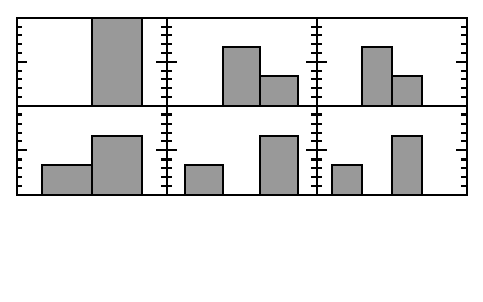
\includegraphics{plots/spark-mc}}%
    \gplfronttext
  \end{picture}%
\endgroup

        \vspace{-5ex}

        (a) \bench{mc}
        \vspace{2ex}

        % GNUPLOT: LaTeX picture with Postscript
\begingroup
\sffamily \footnotesize
  \makeatletter
  \providecommand\color[2][]{%
    \GenericError{(gnuplot) \space\space\space\@spaces}{%
      Package color not loaded in conjunction with
      terminal option `colourtext'%
    }{See the gnuplot documentation for explanation.%
    }{Either use 'blacktext' in gnuplot or load the package
      color.sty in LaTeX.}%
    \renewcommand\color[2][]{}%
  }%
  \providecommand\includegraphics[2][]{%
    \GenericError{(gnuplot) \space\space\space\@spaces}{%
      Package graphicx or graphics not loaded%
    }{See the gnuplot documentation for explanation.%
    }{The gnuplot epslatex terminal needs graphicx.sty or graphics.sty.}%
    \renewcommand\includegraphics[2][]{}%
  }%
  \providecommand\rotatebox[2]{#2}%
  \@ifundefined{ifGPcolor}{%
    \newif\ifGPcolor
    \GPcolorfalse
  }{}%
  \@ifundefined{ifGPblacktext}{%
    \newif\ifGPblacktext
    \GPblacktexttrue
  }{}%
  % define a \g@addto@macro without @ in the name:
  \let\gplgaddtomacro\g@addto@macro
  % define empty templates for all commands taking text:
  \gdef\gplbacktext{}%
  \gdef\gplfronttext{}%
  \makeatother
  \ifGPblacktext
    % no textcolor at all
    \def\colorrgb#1{}%
    \def\colorgray#1{}%
  \else
    % gray or color?
    \ifGPcolor
      \def\colorrgb#1{\color[rgb]{#1}}%
      \def\colorgray#1{\color[gray]{#1}}%
      \expandafter\def\csname LTw\endcsname{\color{white}}%
      \expandafter\def\csname LTb\endcsname{\color{black}}%
      \expandafter\def\csname LTa\endcsname{\color{black}}%
      \expandafter\def\csname LT0\endcsname{\color[rgb]{1,0,0}}%
      \expandafter\def\csname LT1\endcsname{\color[rgb]{0,1,0}}%
      \expandafter\def\csname LT2\endcsname{\color[rgb]{0,0,1}}%
      \expandafter\def\csname LT3\endcsname{\color[rgb]{1,0,1}}%
      \expandafter\def\csname LT4\endcsname{\color[rgb]{0,1,1}}%
      \expandafter\def\csname LT5\endcsname{\color[rgb]{1,1,0}}%
      \expandafter\def\csname LT6\endcsname{\color[rgb]{0,0,0}}%
      \expandafter\def\csname LT7\endcsname{\color[rgb]{1,0.3,0}}%
      \expandafter\def\csname LT8\endcsname{\color[rgb]{0.5,0.5,0.5}}%
    \else
      % gray
      \def\colorrgb#1{\color{black}}%
      \def\colorgray#1{\color[gray]{#1}}%
      \expandafter\def\csname LTw\endcsname{\color{white}}%
      \expandafter\def\csname LTb\endcsname{\color{black}}%
      \expandafter\def\csname LTa\endcsname{\color{black}}%
      \expandafter\def\csname LT0\endcsname{\color{black}}%
      \expandafter\def\csname LT1\endcsname{\color{black}}%
      \expandafter\def\csname LT2\endcsname{\color{black}}%
      \expandafter\def\csname LT3\endcsname{\color{black}}%
      \expandafter\def\csname LT4\endcsname{\color{black}}%
      \expandafter\def\csname LT5\endcsname{\color{black}}%
      \expandafter\def\csname LT6\endcsname{\color{black}}%
      \expandafter\def\csname LT7\endcsname{\color{black}}%
      \expandafter\def\csname LT8\endcsname{\color{black}}%
    \fi
  \fi
  \setlength{\unitlength}{0.0500bp}%
  \begin{picture}(4320.00,2590.00)%
    \gplgaddtomacro\gplbacktext{%
      \csname LTb\endcsname%
      \put(-132,1726){\makebox(0,0)[r]{\strut{}}}%
      \put(-132,2147){\makebox(0,0)[r]{\strut{}}}%
      \put(-132,2567){\makebox(0,0)[r]{\strut{}}}%
      \put(-97,2146){\rotatebox{-270}{\makebox(0,0){\strut{}rounded}}}%
    }%
    \gplgaddtomacro\gplfronttext{%
    }%
    \gplgaddtomacro\gplbacktext{%
      \csname LTb\endcsname%
      \put(1308,1726){\makebox(0,0)[r]{\strut{}}}%
      \put(1308,2147){\makebox(0,0)[r]{\strut{}}}%
      \put(1308,2567){\makebox(0,0)[r]{\strut{}}}%
    }%
    \gplgaddtomacro\gplfronttext{%
    }%
    \gplgaddtomacro\gplbacktext{%
      \csname LTb\endcsname%
      \put(2748,1726){\makebox(0,0)[r]{\strut{}}}%
      \put(2748,2147){\makebox(0,0)[r]{\strut{}}}%
      \put(2748,2567){\makebox(0,0)[r]{\strut{}}}%
    }%
    \gplgaddtomacro\gplfronttext{%
    }%
    \gplgaddtomacro\gplbacktext{%
      \csname LTb\endcsname%
      \put(-132,863){\makebox(0,0)[r]{\strut{}}}%
      \put(-132,1295){\makebox(0,0)[r]{\strut{}}}%
      \put(-132,1726){\makebox(0,0)[r]{\strut{}}}%
      \put(480,731){\rotatebox{-45}{\makebox(0,0)[l]{\strut{}0.99}}}%
      \put(959,731){\rotatebox{-45}{\makebox(0,0)[l]{\strut{}1.0}}}%
      \put(-97,1294){\rotatebox{-270}{\makebox(0,0){\strut{}solved}}}%
    }%
    \gplgaddtomacro\gplfronttext{%
    }%
    \gplgaddtomacro\gplbacktext{%
      \csname LTb\endcsname%
      \put(1308,863){\makebox(0,0)[r]{\strut{}}}%
      \put(1308,1295){\makebox(0,0)[r]{\strut{}}}%
      \put(1308,1726){\makebox(0,0)[r]{\strut{}}}%
      \put(1800,731){\rotatebox{-45}{\makebox(0,0)[l]{\strut{}0.99}}}%
      \put(2160,731){\rotatebox{-45}{\makebox(0,0)[l]{\strut{}0.999}}}%
      \put(2519,731){\rotatebox{-45}{\makebox(0,0)[l]{\strut{}1.0}}}%
    }%
    \gplgaddtomacro\gplfronttext{%
    }%
    \gplgaddtomacro\gplbacktext{%
      \csname LTb\endcsname%
      \put(2748,863){\makebox(0,0)[r]{\strut{}}}%
      \put(2748,1295){\makebox(0,0)[r]{\strut{}}}%
      \put(2748,1726){\makebox(0,0)[r]{\strut{}}}%
      \put(3168,731){\rotatebox{-45}{\makebox(0,0)[l]{\strut{}0.99}}}%
      \put(3456,731){\rotatebox{-45}{\makebox(0,0)[l]{\strut{}0.999}}}%
      \put(3743,731){\rotatebox{-45}{\makebox(0,0)[l]{\strut{}0.9999}}}%
      \put(4031,731){\rotatebox{-45}{\makebox(0,0)[l]{\strut{}1.0}}}%
    }%
    \gplgaddtomacro\gplfronttext{%
    }%
    \gplbacktext
    \put(0,0){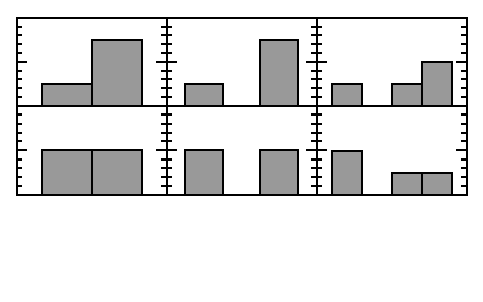
\includegraphics{plots/spark-simpleRaytracer}}%
    \gplfronttext
  \end{picture}%
\endgroup

        \vspace{-5ex}

        (b) \bench{raytracer}

    \caption{Sensitivity to hardware restrictions for two representative benchmarks. The
    horizontal axes show the probability levels while the vertical axes
    reflect the fraction of all approximate operations in an execution
    assigned to each level. The \emph{rounded} executions were assigned to levels
    after solving without restrictions; the \emph{solved} executions used the
    hardware profile during type inference.}
    \label{fig:spark}
\end{figure}

To run a \lang-compiled program on realistic approximate hardware, two
strategies are possible for selecting the probability level for each operation.
A simplistic approach rounds the inferred probabilities up to the nearest
level.
The compiler can potentially do better by using the SMT solver to apply hardware
constraints during type inference if the deployment architecture is known
ahead of time.

Figure~\ref{fig:spark} compares the two approaches, denoted \emph{solving} and
\emph{rounding},
for two of
our benchmarks on \mbox{two-,} \mbox{three-,} and four-level machines.
Hardware-constrained solving shifts the distribution toward lower
probabilities in each of the three machines.
When \bench{mc} runs on a three-level machine, for example, the simple
rounding strategy rarely uses the lowest $p=0.99$ reliability level;
if we instead inform the solver that this level is available, the benchmark
can use it for a third of its approximate operations.
A similar effect arises for \bench{raytracer}, for which the solver assigns the
lowest reliability level to about half of the operations executed while
rounding makes the majority of operations fully reliable.

These differences suggest that optimizing an approximate program for a
specific hardware configuration can enable significant energy savings,
\emph{even for simple approximate machines with only two probability levels}.
\lang's solver-based tuning approach enables this kind of
optimization.
% freeing programmers from the need to manually reason about the complex
% interaction between local operator-probability decisions.

While solving for hardware constraints can lead to better efficiency at run
time, it can also be more expensive at compile time.
The SMT queries for most benchmarks took only a few minutes,
but two outliers---\code{sor} and \code{zxing}---took much longer when level constraints
were enabled.
For \code{sor}, solving succeeded for machine configurations up to four levels
but exceeded a 30-minute timeout for larger level counts;
\code{zxing} timed out even in the two-level configuration.
In the remainder of this evaluation, we use the more sophisticated solving
scheme, except for these cases where solving times out and we fall back to the
cheaper rounding strategy.


\paragraph{Probability granularity.}

\begin{figure*}
    \hspace{-3ex}
    % GNUPLOT: LaTeX picture with Postscript
\begingroup
\sffamily \footnotesize
  \makeatletter
  \providecommand\color[2][]{%
    \GenericError{(gnuplot) \space\space\space\@spaces}{%
      Package color not loaded in conjunction with
      terminal option `colourtext'%
    }{See the gnuplot documentation for explanation.%
    }{Either use 'blacktext' in gnuplot or load the package
      color.sty in LaTeX.}%
    \renewcommand\color[2][]{}%
  }%
  \providecommand\includegraphics[2][]{%
    \GenericError{(gnuplot) \space\space\space\@spaces}{%
      Package graphicx or graphics not loaded%
    }{See the gnuplot documentation for explanation.%
    }{The gnuplot epslatex terminal needs graphicx.sty or graphics.sty.}%
    \renewcommand\includegraphics[2][]{}%
  }%
  \providecommand\rotatebox[2]{#2}%
  \@ifundefined{ifGPcolor}{%
    \newif\ifGPcolor
    \GPcolorfalse
  }{}%
  \@ifundefined{ifGPblacktext}{%
    \newif\ifGPblacktext
    \GPblacktexttrue
  }{}%
  % define a \g@addto@macro without @ in the name:
  \let\gplgaddtomacro\g@addto@macro
  % define empty templates for all commands taking text:
  \gdef\gplbacktext{}%
  \gdef\gplfronttext{}%
  \makeatother
  \ifGPblacktext
    % no textcolor at all
    \def\colorrgb#1{}%
    \def\colorgray#1{}%
  \else
    % gray or color?
    \ifGPcolor
      \def\colorrgb#1{\color[rgb]{#1}}%
      \def\colorgray#1{\color[gray]{#1}}%
      \expandafter\def\csname LTw\endcsname{\color{white}}%
      \expandafter\def\csname LTb\endcsname{\color{black}}%
      \expandafter\def\csname LTa\endcsname{\color{black}}%
      \expandafter\def\csname LT0\endcsname{\color[rgb]{1,0,0}}%
      \expandafter\def\csname LT1\endcsname{\color[rgb]{0,1,0}}%
      \expandafter\def\csname LT2\endcsname{\color[rgb]{0,0,1}}%
      \expandafter\def\csname LT3\endcsname{\color[rgb]{1,0,1}}%
      \expandafter\def\csname LT4\endcsname{\color[rgb]{0,1,1}}%
      \expandafter\def\csname LT5\endcsname{\color[rgb]{1,1,0}}%
      \expandafter\def\csname LT6\endcsname{\color[rgb]{0,0,0}}%
      \expandafter\def\csname LT7\endcsname{\color[rgb]{1,0.3,0}}%
      \expandafter\def\csname LT8\endcsname{\color[rgb]{0.5,0.5,0.5}}%
    \else
      % gray
      \def\colorrgb#1{\color{black}}%
      \def\colorgray#1{\color[gray]{#1}}%
      \expandafter\def\csname LTw\endcsname{\color{white}}%
      \expandafter\def\csname LTb\endcsname{\color{black}}%
      \expandafter\def\csname LTa\endcsname{\color{black}}%
      \expandafter\def\csname LT0\endcsname{\color{black}}%
      \expandafter\def\csname LT1\endcsname{\color{black}}%
      \expandafter\def\csname LT2\endcsname{\color{black}}%
      \expandafter\def\csname LT3\endcsname{\color{black}}%
      \expandafter\def\csname LT4\endcsname{\color{black}}%
      \expandafter\def\csname LT5\endcsname{\color{black}}%
      \expandafter\def\csname LT6\endcsname{\color{black}}%
      \expandafter\def\csname LT7\endcsname{\color{black}}%
      \expandafter\def\csname LT8\endcsname{\color{black}}%
    \fi
  \fi
  \setlength{\unitlength}{0.0500bp}%
  \begin{picture}(12960.00,3888.00)%
    \gplgaddtomacro\gplbacktext{%
      \csname LTb\endcsname%
      \put(858,440){\makebox(0,0)[r]{\strut{}0\%}}%
      \put(858,1077){\makebox(0,0)[r]{\strut{}20\%}}%
      \put(858,1713){\makebox(0,0)[r]{\strut{}40\%}}%
      \put(858,2350){\makebox(0,0)[r]{\strut{}60\%}}%
      \put(858,2986){\makebox(0,0)[r]{\strut{}80\%}}%
      \put(858,3623){\makebox(0,0)[r]{\strut{}100\%}}%
      \put(1266,220){\makebox(0,0){\strut{}2}}%
      \put(1376,220){\makebox(0,0){\strut{}3}}%
      \put(1486,220){\makebox(0,0){\strut{}4}}%
      \put(1597,220){\makebox(0,0){\strut{}5}}%
      \put(1707,220){\makebox(0,0){\strut{}6}}%
      \put(1817,220){\makebox(0,0){\strut{}7}}%
      \put(1927,220){\makebox(0,0){\strut{}8}}%
      \put(2148,220){\makebox(0,0){\strut{}2}}%
      \put(2258,220){\makebox(0,0){\strut{}3}}%
      \put(2368,220){\makebox(0,0){\strut{}4}}%
      \put(2479,220){\makebox(0,0){\strut{}5}}%
      \put(2589,220){\makebox(0,0){\strut{}6}}%
      \put(2699,220){\makebox(0,0){\strut{}7}}%
      \put(2810,220){\makebox(0,0){\strut{}8}}%
      \put(3030,220){\makebox(0,0){\strut{}2}}%
      \put(3140,220){\makebox(0,0){\strut{}3}}%
      \put(3251,220){\makebox(0,0){\strut{}4}}%
      \put(3361,220){\makebox(0,0){\strut{}5}}%
      \put(3471,220){\makebox(0,0){\strut{}6}}%
      \put(3581,220){\makebox(0,0){\strut{}7}}%
      \put(3692,220){\makebox(0,0){\strut{}8}}%
      \put(3912,220){\makebox(0,0){\strut{}2}}%
      \put(4023,220){\makebox(0,0){\strut{}3}}%
      \put(4133,220){\makebox(0,0){\strut{}4}}%
      \put(4243,220){\makebox(0,0){\strut{}5}}%
      \put(4353,220){\makebox(0,0){\strut{}6}}%
      \put(4464,220){\makebox(0,0){\strut{}7}}%
      \put(4574,220){\makebox(0,0){\strut{}8}}%
      \put(4794,220){\makebox(0,0){\strut{}2}}%
      \put(4905,220){\makebox(0,0){\strut{}3}}%
      \put(5015,220){\makebox(0,0){\strut{}4}}%
      \put(5125,220){\makebox(0,0){\strut{}5}}%
      \put(5236,220){\makebox(0,0){\strut{}6}}%
      \put(5346,220){\makebox(0,0){\strut{}7}}%
      \put(5456,220){\makebox(0,0){\strut{}8}}%
      \put(5677,220){\makebox(0,0){\strut{}2}}%
      \put(5787,220){\makebox(0,0){\strut{}3}}%
      \put(5897,220){\makebox(0,0){\strut{}4}}%
      \put(6008,220){\makebox(0,0){\strut{}5}}%
      \put(6118,220){\makebox(0,0){\strut{}6}}%
      \put(6228,220){\makebox(0,0){\strut{}7}}%
      \put(6338,220){\makebox(0,0){\strut{}8}}%
      \put(6559,220){\makebox(0,0){\strut{}2}}%
      \put(6669,220){\makebox(0,0){\strut{}3}}%
      \put(6779,220){\makebox(0,0){\strut{}4}}%
      \put(6890,220){\makebox(0,0){\strut{}\raisebox{1.5ex}{\shortstack{$\star$\\5}}}}%
      \put(7000,220){\makebox(0,0){\strut{}\raisebox{1.5ex}{\shortstack{$\star$\\6}}}}%
      \put(7110,220){\makebox(0,0){\strut{}\raisebox{1.5ex}{\shortstack{$\star$\\7}}}}%
      \put(7221,220){\makebox(0,0){\strut{}\raisebox{1.5ex}{\shortstack{$\star$\\8}}}}%
      \put(7441,220){\makebox(0,0){\strut{}\raisebox{1.5ex}{\shortstack{$\star$\\2}}}}%
      \put(7551,220){\makebox(0,0){\strut{}\raisebox{1.5ex}{\shortstack{$\star$\\3}}}}%
      \put(7662,220){\makebox(0,0){\strut{}\raisebox{1.5ex}{\shortstack{$\star$\\4}}}}%
      \put(7772,220){\makebox(0,0){\strut{}\raisebox{1.5ex}{\shortstack{$\star$\\5}}}}%
      \put(7882,220){\makebox(0,0){\strut{}\raisebox{1.5ex}{\shortstack{$\star$\\6}}}}%
      \put(7992,220){\makebox(0,0){\strut{}\raisebox{1.5ex}{\shortstack{$\star$\\7}}}}%
      \put(8103,220){\makebox(0,0){\strut{}\raisebox{1.5ex}{\shortstack{$\star$\\8}}}}%
    }%
    \gplgaddtomacro\gplfronttext{%
      \csname LTb\endcsname%
      \put(9332,3513){\makebox(0,0)[l]{\strut{}0.99}}%
      \csname LTb\endcsname%
      \put(9332,3293){\makebox(0,0)[l]{\strut{}0.999}}%
      \csname LTb\endcsname%
      \put(9332,3073){\makebox(0,0)[l]{\strut{}0.9999}}%
      \csname LTb\endcsname%
      \put(9332,2853){\makebox(0,0)[l]{\strut{}0.99999}}%
      \csname LTb\endcsname%
      \put(9332,2633){\makebox(0,0)[l]{\strut{}0.999999}}%
      \csname LTb\endcsname%
      \put(9332,2413){\makebox(0,0)[l]{\strut{}0.9999999}}%
      \csname LTb\endcsname%
      \put(9332,2193){\makebox(0,0)[l]{\strut{}0.99999999}}%
      \csname LTb\endcsname%
      \put(9332,1973){\makebox(0,0)[l]{\strut{}1.0}}%
      \csname LTb\endcsname%
      \put(7772,99){\makebox(0,0){\strut{}\raisebox{-2ex}{zxing}}}%
      \put(6890,99){\makebox(0,0){\strut{}\raisebox{-2ex}{sor}}}%
      \put(6008,99){\makebox(0,0){\strut{}\raisebox{-2ex}{smm}}}%
      \put(5125,99){\makebox(0,0){\strut{}\raisebox{-2ex}{raytracer}}}%
      \put(4243,99){\makebox(0,0){\strut{}\raisebox{-2ex}{mc}}}%
      \put(3361,99){\makebox(0,0){\strut{}\raisebox{-2ex}{lu}}}%
      \put(2479,99){\makebox(0,0){\strut{}\raisebox{-2ex}{imagefill}}}%
      \put(1597,99){\makebox(0,0){\strut{}\raisebox{-2ex}{fft}}}%
    }%
    \gplbacktext
    \put(0,0){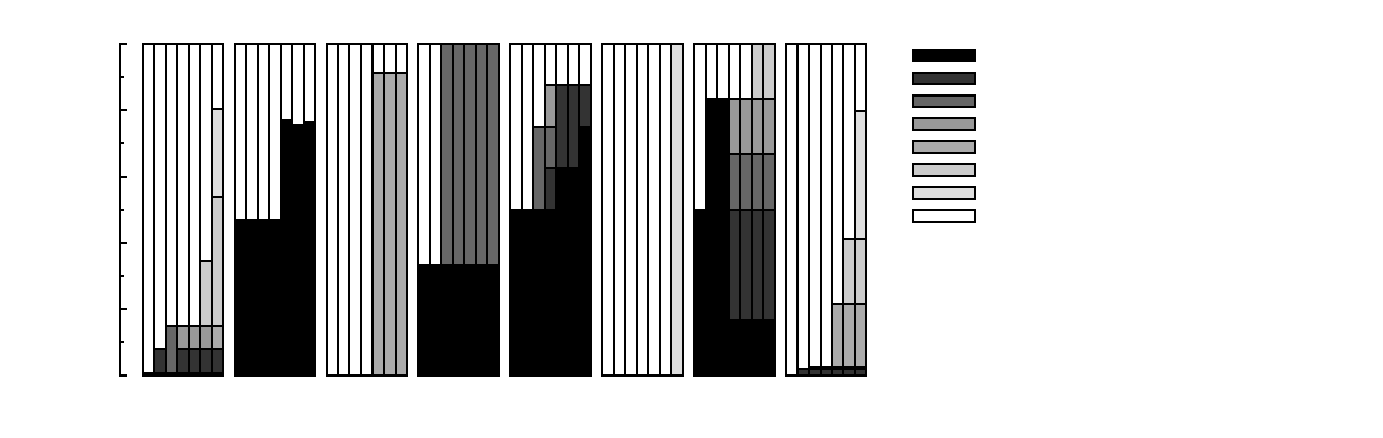
\includegraphics{plots/levelbreakdown}}%
    \gplfronttext
  \end{picture}%
\endgroup

    \caption{Operator probability breakdowns. Each bar shows a hardware
    configuration with a different number of levels.
    Darker shades indicate lower probabilities and correspondingly higher
    potential energy savings.
    Bars marked $\star$ used
    the cheaper rounding strategy instead of solving to determine levels.}
    \label{fig:levels}
\end{figure*}

More hardware probability levels can enable greater efficiency gains by
closely matching applications' probability requirements.
Figure~\ref{fig:levels} depicts the allocation of approximate operations in benchmark
executions to reliability levels for a range of hardware configurations
from 2 to 8 levels.
In this graphic, white and lighter shades indicate more reliable execution and
correspondingly lower efficiency gains; darker shades indicate more
opportunity for energy savings.

Five of the eight benchmarks use multiple operator probability levels below
1.0 when optimized for hardware that offers this flexibility.
This suggests that multi-level approximate hardware designs like
QUORA~\cite{quora} can unlock more efficiency gains in these benchmarks than simpler
single-probability machines like Truffle~\cite{truffle}.
The exceptions are \code{imagefill}, \code{lu}, and \code{smm}, where a single
probability level seems to suffice for the majority of operations.

Most of our benchmarks exhibit a diminishing returns after a certain number of
levels.
For example, \bench{mc} increases its amount of approximation up to four levels
but does not benefit from higher level counts.
Similarly, \bench{imagefill}'s benefits do not increase after six levels.
In contrast, \bench{raytracer} and \bench{zxing} see improvements
for configurations up to eight levels.

In an extreme case, \bench{smm} falls back to reliable execution for nearly all
of its operations in every configuration we simulated except for the
eight-level machine.
This suggests that a two-level machine would suffice for this benchmark,
provided the single approximate operation probability were high enough.
On the other hand, specializing a two-level architecture to this outlier
would limit potential efficiency gains for other applications.

Increasing reliability levels do not strictly lead to efficiency benefits in
\lang's solver-based approach.
For \bench{sor}, the added constraints for more granular hardware levels lead
to a more complex SMT solver query and eventually timeouts.
After four levels, the solver failed to optimize the benchmark and we fell back
to the na\"ive rounding strategy, which leads to lower efficiency gains.
These timeouts are partially due to \lang's straightforward encoding of
program and hardware constraints;
future work on optimizing \lang's constraint systems for efficient solving
could make larger level counts more tractable.


\paragraph{Comparison to ideal.}

\begin{figure}
    \hspace{-3ex}
    % GNUPLOT: LaTeX picture with Postscript
\begingroup
\sffamily \footnotesize
  \makeatletter
  \providecommand\color[2][]{%
    \GenericError{(gnuplot) \space\space\space\@spaces}{%
      Package color not loaded in conjunction with
      terminal option `colourtext'%
    }{See the gnuplot documentation for explanation.%
    }{Either use 'blacktext' in gnuplot or load the package
      color.sty in LaTeX.}%
    \renewcommand\color[2][]{}%
  }%
  \providecommand\includegraphics[2][]{%
    \GenericError{(gnuplot) \space\space\space\@spaces}{%
      Package graphicx or graphics not loaded%
    }{See the gnuplot documentation for explanation.%
    }{The gnuplot epslatex terminal needs graphicx.sty or graphics.sty.}%
    \renewcommand\includegraphics[2][]{}%
  }%
  \providecommand\rotatebox[2]{#2}%
  \@ifundefined{ifGPcolor}{%
    \newif\ifGPcolor
    \GPcolorfalse
  }{}%
  \@ifundefined{ifGPblacktext}{%
    \newif\ifGPblacktext
    \GPblacktexttrue
  }{}%
  % define a \g@addto@macro without @ in the name:
  \let\gplgaddtomacro\g@addto@macro
  % define empty templates for all commands taking text:
  \gdef\gplbacktext{}%
  \gdef\gplfronttext{}%
  \makeatother
  \ifGPblacktext
    % no textcolor at all
    \def\colorrgb#1{}%
    \def\colorgray#1{}%
  \else
    % gray or color?
    \ifGPcolor
      \def\colorrgb#1{\color[rgb]{#1}}%
      \def\colorgray#1{\color[gray]{#1}}%
      \expandafter\def\csname LTw\endcsname{\color{white}}%
      \expandafter\def\csname LTb\endcsname{\color{black}}%
      \expandafter\def\csname LTa\endcsname{\color{black}}%
      \expandafter\def\csname LT0\endcsname{\color[rgb]{1,0,0}}%
      \expandafter\def\csname LT1\endcsname{\color[rgb]{0,1,0}}%
      \expandafter\def\csname LT2\endcsname{\color[rgb]{0,0,1}}%
      \expandafter\def\csname LT3\endcsname{\color[rgb]{1,0,1}}%
      \expandafter\def\csname LT4\endcsname{\color[rgb]{0,1,1}}%
      \expandafter\def\csname LT5\endcsname{\color[rgb]{1,1,0}}%
      \expandafter\def\csname LT6\endcsname{\color[rgb]{0,0,0}}%
      \expandafter\def\csname LT7\endcsname{\color[rgb]{1,0.3,0}}%
      \expandafter\def\csname LT8\endcsname{\color[rgb]{0.5,0.5,0.5}}%
    \else
      % gray
      \def\colorrgb#1{\color{black}}%
      \def\colorgray#1{\color[gray]{#1}}%
      \expandafter\def\csname LTw\endcsname{\color{white}}%
      \expandafter\def\csname LTb\endcsname{\color{black}}%
      \expandafter\def\csname LTa\endcsname{\color{black}}%
      \expandafter\def\csname LT0\endcsname{\color{black}}%
      \expandafter\def\csname LT1\endcsname{\color{black}}%
      \expandafter\def\csname LT2\endcsname{\color{black}}%
      \expandafter\def\csname LT3\endcsname{\color{black}}%
      \expandafter\def\csname LT4\endcsname{\color{black}}%
      \expandafter\def\csname LT5\endcsname{\color{black}}%
      \expandafter\def\csname LT6\endcsname{\color{black}}%
      \expandafter\def\csname LT7\endcsname{\color{black}}%
      \expandafter\def\csname LT8\endcsname{\color{black}}%
    \fi
  \fi
  \setlength{\unitlength}{0.0500bp}%
  \begin{picture}(5040.00,3888.00)%
    \gplgaddtomacro\gplbacktext{%
      \csname LTb\endcsname%
      \put(660,440){\makebox(0,0)[r]{\strut{}0\%}}%
      \put(660,909){\makebox(0,0)[r]{\strut{}20\%}}%
      \put(660,1379){\makebox(0,0)[r]{\strut{}40\%}}%
      \put(660,1848){\makebox(0,0)[r]{\strut{}60\%}}%
      \put(660,2318){\makebox(0,0)[r]{\strut{}80\%}}%
      \put(660,2787){\makebox(0,0)[r]{\strut{}100\%}}%
      \put(1135,220){\makebox(0,0){\strut{}fft}}%
      \put(1625,220){\makebox(0,0){\strut{}imagefill}}%
      \put(2115,220){\makebox(0,0){\strut{}lu}}%
      \put(2605,220){\makebox(0,0){\strut{}mc}}%
      \put(3094,220){\makebox(0,0){\strut{}raytracer}}%
      \put(3584,220){\makebox(0,0){\strut{}smm}}%
      \put(4074,220){\makebox(0,0){\strut{}sor}}%
      \put(4564,220){\makebox(0,0){\strut{}zxing}}%
    }%
    \gplgaddtomacro\gplfronttext{%
      \csname LTb\endcsname%
      \put(1251,3055){\makebox(0,0)[l]{\strut{}$p<0.99$}}%
      \csname LTb\endcsname%
      \put(1251,3275){\makebox(0,0)[l]{\strut{}$0.99 \le p < 0.99999999$}}%
      \csname LTb\endcsname%
      \put(1251,3495){\makebox(0,0)[l]{\strut{}$0.99999999 \le p < 1.0$}}%
      \csname LTb\endcsname%
      \put(1251,3715){\makebox(0,0)[l]{\strut{}$p=1.0$}}%
    }%
    \gplbacktext
    \put(0,0){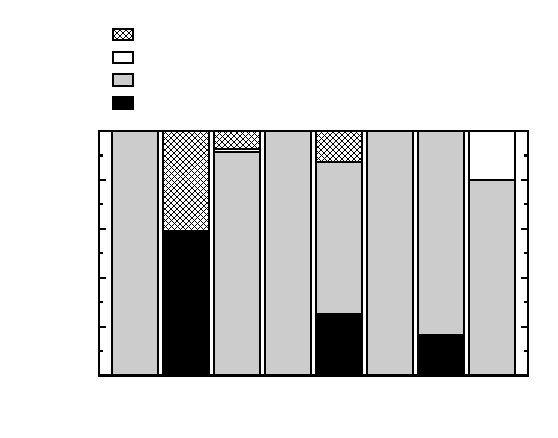
\includegraphics{plots/idealhist}}%
    \gplfronttext
  \end{picture}%
\endgroup

    \caption{Approximate operation probabilities on an ideal continuous
    machine. The gray boxes show the probability range accommodated by
    our simulated discrete-level machines, while the white box represents
    higher-reliability operations and the black boxes are
    lower-reliability operations.
    The hatched box indicates approximate operations that are forced to
    execute reliably by program constraints, even on ideal hardware.}
    \label{fig:idealhist}
\end{figure}

An ideal approximate architecture that features arbitrary probability levels
could offer more flexibility at the extremes of the probability range.
To evaluate the importance of higher and lower levels, we
simulated an ideal continuous machine.
Figure~\ref{fig:idealhist} shows the fraction of approximate operations in
executions of each benchmark that used probabilities below the range of our
realistic machines (below 99\% probability) and above the range (above $p =
1.0 - 10^{-8}$).
The figure also shows the operations that executed with probability exactly
1.0 even on this continuous architecture, indicating that they were
constrained by program requirements rather than hardware limitations.

For all but one application, most operations lie in the range of probabilities
offered by our discrete machine simulations.
Only three benchmarks show a significant number of operations with
probabilities below 99\%, and one outlier, \code{imagefill}, uses these
low-probability operations for nearly all of its approximable computations.
The only benchmark that significantly uses higher-probability operations
is \code{zxing}, where about 20\% of the operations executed had a probability
greater than $1.0 - 10^{-8}$.
Among our benchmarks, the $0.99 \le p \le 0.99999999$ probability range
suffices to capture most of the flexibility offered by an ideal machine.


\paragraph{Example energy model.}
This evaluation measures error probabilities with the goal of allowing
hardware designers to plug in energy models.
(We intend to make the raw data available in full after publication.)
To give a sense of the potential savings, we apply a simple energy model
based on EnerJ~\cite{enerj}: a correctness probability of 0.99 yields 30\%
energy savings over a precise operation, $p=10^{-4}$ saves 20\%, $p=10^{-6}$
saves 10\%, and other levels are interpolated.
More optimistic hardware proposals exist (e.g., \citet{quora}), but EnerJ's
conservative CPU-based model serves as a useful point of comparison.
On an eight-level machine, the total operation energy saved for each
benchmark is:
%
\begin{center}
\edef\energy#1{\ifstrequal{#1}{fft-solved}{$<$1\%}{\ifstrequal{#1}{imagefill-rounded}{7\%}{\ifstrequal{#1}{imagefill-solved}{22\%}{\ifstrequal{#1}{lu-rounded}{$<$1\%}{\ifstrequal{#1}{lu-solved}{9\%}{\ifstrequal{#1}{mc-rounded}{5\%}{\ifstrequal{#1}{mc-solved}{23\%}{\ifstrequal{#1}{simpleRaytracer-rounded}{1\%}{\ifstrequal{#1}{simpleRaytracer-solved}{20\%}{\ifstrequal{#1}{smm-rounded}{2\%}{\ifstrequal{#1}{smm-solved}{2\%}{\ifstrequal{#1}{sor-rounded}{12\%}{\ifstrequal{#1}{sor-solved}{---}{\ifstrequal{#1}{zxing-rounded}{1\%}{\ifstrequal{#1}{zxing-solved}{---}{\errmessage{unknown key for energy: #1}}}}}}}}}}}}}}}}}}

\begin{tabular}{l r r}
\toprule
Benchmark & Rounded & Solved \\
\midrule
\bench{fft} & \energy{fft-rounded} & \energy{fft-solved} \\
\bench{imagefill} & \energy{imagefill-rounded} & \energy{imagefill-solved} \\
\bench{lu} & \energy{lu-rounded} & \energy{lu-solved} \\
\bench{mc} & \energy{mc-rounded} & \energy{mc-solved} \\
\bench{raytracer} & \energy{simpleRaytracer-rounded} & \energy{simpleRaytracer-solved} \\
\bench{smm} & \energy{smm-rounded} & \energy{smm-solved} \\
\bench{sor} & \energy{sor-rounded} & \energy{sor-solved} \\
\bench{zxing} & \energy{zxing-rounded} & \energy{zxing-solved} \\
\bottomrule
\end{tabular}
\end{center}
%
The table shows the modeled energy reduction for both the hardware-oblivious
rounding strategy and the platform-specific solving strategy (except where the
solver timed out).
The results reflect the above finding that solving yields better savings than
rounding after the fact.


\subsection{Interprocedural Inference and Specialization}

In all of our benchmarks, we used the inferred \code{@Approx} qualifier on
function parameters and return types to let the compiler propagate constraints
interprocedurally.
This let us write simpler annotations that directly encoded our desired output
correctness constraints and avoid artificially aligning them with function
boundaries.
In some benchmarks---namely, \bench{lu} and \bench{zxing}---multiple call
sites to these inferred functions allowed the compiler to specialize variants
and improve efficiency.

In \bench{lu}, for example, specialization was critical to making the
benchmark take advantage of approximate hardware.
That benchmark uses a utility function that copies approximate arrays.
The factorization routine has three calls to the copying function, and each of
the intermediate arrays involved have varying impact on the output of the
benchmark.
When we limit the program to $k=1$ function variants---disabling function
specialization---all three of these intermediates are constrained to
have identical correctness probability, and all three must be as reliable as
the least tolerant among them.
As a result, the benchmark as a whole exhibits very little approximate
execution: more than 99\% of its approximate operations are executed reliably
($p = 1.0$).
By allowing $k=2$ function specializations, however, the compiler reduces the
fraction to 8\%, and $k=3$ specializations further reduce it to 7\%.
A similar pattern arises in the \bench{zxing} benchmark, where utility functions
on its central data structure---a bit-matrix class used to hold
black-and-white pixel values---are invoked from different contexts
throughout the program.


\subsection{Dynamic Tracking}

The \code{@Dyn} type qualifier lets programmers request dynamic
probability tracking, in exchange for run-time overhead, when \lang's static
tracking is too conservative.
Table~\ref{table:bench} shows the number of types we annotated with
\code{@Dyn} in each benchmark.
Dynamic tracking was necessary at least once in every benchmark except one
(\code{imagefill}).
Most commonly, \code{@Dyn} applied in loops that accumulate approximate
values.
For example, \code{zxing} has a loop that searches for image patterns that
suggest the presence of parts of a QR code.
The actual detection of each pattern can be statically tracked, but the loop
also accumulates the total size of the image patterns.
Since the loop's trip count depends on the input image, dynamic tracking was
necessary for precision:
no nonzero static bound on the size variable's probability would suffice.

Table~\ref{table:bench} also shows the fraction of operations in an execution
of each benchmark that required dynamic tracking.
In five of our eight benchmarks, less than 1\% of the operations in the
program need to be dynamically tracked, suggesting that energy overhead would
be minimal.
In the remaining three benchmarks, a significant portion of the application's
approximate and reliable operations required dynamic tracking.
(Recall that operations on \code{@Dyn}-typed variables are reliable by default
but still require propagation of probability information.)
In the worst case, \code{fft} uses dynamic tracking for \dynops{fft-dyn} of
the operations in its execution.

In a simple implementation, each dynamically tracked operation expands out to
two operations, so
the percentage of dynamically tracked operations is equivalent to the
overhead incurred.
An optimizing compiler, however, can likely coalesce and strength-reduce the
multiplications-by-constants that make up tracking code.
In \code{fft}, for example, an inner loop reads two array elements, updates
them each with a series of four approximate operations, and writes them back.
A standard constant-propagation optimization could coalesce the four tracking
operations to a single update.
In other cases, such as \code{zxing}'s pattern-search loop described above,
the correctness probability loss is directly proportional to the loop trip
count.
Standard loop optimizations could hoist these updates out of the loop and
further reduce overhead.


\subsection{Tool Performance}

Table~\ref{table:bench} lists the running time of the inference system for
each benchmark.
The total time includes time spent on the initial system-satisfiability query,
the optimization query series, parsing and analyzing the Java
source code, and checking for \lang constraint warnings.
Most of the time is spent in optimization, so it can be faster to produce a
satisfying but suboptimal type assignment.
The optimization queries have a timeout of one minute, so the final SMT query
in the series can take at most this long; for several benchmarks, the solver
returns \emph{unsatisfiable} before this timeout is reached.
The compiler typically runs in about 1--20~minutes.
One outlier is \code{fft}, whose constraint system is fast to solve because of
the benchmark's reliance on dynamic tracking.

These measurements are for a continuous configuration of the system rather
than a more expensive level-constrained version.
Solver times for hardware-constrained inference are comparable, except for the
two benchmarks mentioned above that scale poorly and eventually time out:
\code{sor} and \code{zxing}.




\section{Related Work}

Programming systems for approximate computing have recently become an area of
interest for programming languages research.
This work's primary distinctions are its focus on types for annotation
flexibility,
exploitation of recent multi-level architectures,
and integration of static and dynamic tracking.

Some approaches to approximate programming, including Relax~\cite{relax}
and EnerJ~\cite{enerj}, focus primarily on \emph{safety} properties:
preventing bugs where approximation contaminates pointers or causes wild
control flow.
These proposals have focused on deciding which parts of a computation may be
subject to error.
Our work addresses the related but distinct issue of \emph{quality}, which
concerns the degree of error allowable in a program.

\lang is most closely related to other systems for inferring operator
reliabilities to meet program\-mer-specified correctness bounds.
Chisel~\cite{chisel} uses an integer linear programming formulation
to choose which operations in a function should be made approximate to
meet a bound on the function's return value.
Similarly, ExpAX~\cite{expax-tr} uses a data-flow analysis combined with a
genetic algorithm to determine which operations in a program to approximate
based on an overall quality bound for the entire application.
\lang's type-based approach is new in four important ways:
(1) Where prior work assumes a single level of hardware approximation, \lang
is the first language we are aware of that targets approximate architectures
with multiple probabilities.
We show empirically that multi-level architectures can offer applications
better efficiency for the same output reliability than simpler single-level
approximation.
(2) \lang shows how to augment static guarantees with run-time monitoring.
(3) \lang can specialize functions according to quality demands in calling
contexts.
(4) Probability type qualifiers admit flexible annotation that scales with
programmer effort.

Probabilistic assertions~\cite{passert} express statistical program
properties: for example, output quality requirements in approximate programs.
The verifier supports arbitrary accuracy metrics, but it cannot produce
conservative bounds or infer partially-specified approximations.
Similarly, Bornholt et~al.'s \mbox{Uncertain\textless{T}\textgreater}~\cite{uncertaint} uses a library-based approach to
compose probability distributions at run time, a process that resembles \lang's
dynamic probability tracking.

\lang also relates to systems for optimizing floating-point precision.
Precimonious~\cite{precimonious} chooses bitwidths to meet an output precision
bound, while \citet{stoke-fp} design a superoptimizer that
takes an accurate kernel and
synthesizes new implementations that approximate the original
behavior.

While type inference typically reconstructs types so that any solution leads
to the same program semantics, \lang's inference determines the
program's probabilistic behavior.
Similarly,
Chlorophyll uses type inference to assign data and computations to processing
elements to minimize communication~\cite{chlorophyll}.
That work also uses an SMT solver to optimize an objective function.


\section{Conclusion}

Approximate programming models need tools that help developers decide how much
reliability is necessary throughout an algorithm.
Especially when probabilistic operation is involved, manual reasoning about
individual operator reliabilities can be tedious and error-prone.
On the other hand, fully automatic approaches are also problematic: since
approximation has broad implications for software correctness, programmers
sometimes need fine-grained control over its effects.
An opaque auto-tuner sacrifices programmer visibility and control.
\lang's solver-aided type inference offers an intermediate solution that lets programmers
write constraints only where they are most relevant.
Combined with code specialization and dynamic tracking, \lang gives
programmers flexible control over the efficiency--accuracy trade-offs offered
by approximate hardware.

\ifnum\cameraready=1
\acks
This work was supported in part by C-FAR, one of the six SRC STARnet Centers,
sponsored by MARCO and DARPA, by NSF grant \#1216611, by a Qualcomm Innovation
Fellowship, and by gifts from Microsoft.
\fi

\bibliographystyle{abbrvnat}
\bibliography{approx-within}

\clearpage
\appendix
\section{Full Semantics and Proof}
\label{app:semantics}

This appendix expands on the formalism overview in
Section~\ref{sec:semantics}.
We present the full syntax, static semantics, and dynamic semantics for the
core \lang language.
We prove a \emph{soundness} theorem that embodies the probability type
system's fundamental accuracy guarantee.

\newcommand{\relinput}[1]{
    \IfFileExists{./#1.tex}{\input{#1}}{\input{semantics/#1}}
}

\subsection{Syntax}

We formalize a core of \lang without inference.
The syntax for statements, expressions, and types is:
%
\relinput{syntax}
%
For the purpose of the static and dynamic semantics, we also define values $V$, heaps
$H$, dynamic probability maps $D$, true probability maps $S$, and static
contexts $\Gamma$:
%
\begin{align*}
    V &\defeq
        c \alt
        \Box \\
    H &\defeq
        \cdot \alt
        H, v \mapsto V \\
    D &\defeq
        \cdot \alt
        D, v \mapsto p \\
    S &\defeq
        \cdot \alt
        S, v \mapsto p \\
    \Gamma &\defeq
        \cdot \alt
        \Gamma, v \mapsto T
\end{align*}
%
We define $H(v)$, $D(v)$, $S(v)$, and $\Gamma(v)$ to denote variable lookup in
these maps.


\subsection{Typing}

The type system defines the static semantics for the core language. We first
give typing judgments first for expressions and then for statements.

\subsubsection{Operator Typing}

We introduce a helper ``function'' that determines the unqualified result type
of a binary arithmetic operator.

\vspace{1ex}\noindent
$\boxed{\text{optype}(\tau_1, \tau_2) = \tau_3}$
%
\begin{mathpar}
    \text{optype}(\tau,\tau) = \tau

    \text{optype}(\mcode{int},\mcode{float}) =
           \mcode{float}

    \text{optype}(\mcode{float},\mcode{int}) =
           \mcode{float}
\end{mathpar}
%
Now we can give the types of the binary operator expressions themselves.
There are two cases: one for statically-typed operators and one for
dynamic tracking.
The operands may not mix static and dynamic qualifiers (recall that the
compiler inserts \mcode{track} casts to introduce dynamic tracking when
necessary).

\vspace{1ex}\noindent
$\boxed{\Gamma \vdash e : T}$
%
\begin{mathpar}
    \inferrule[op-static-types]
    {\Gamma \vdash e_1 : \ApproxN{p_1} \> \tau_1 \\
    \Gamma \vdash e_2 : \ApproxN{p_2} \> \tau_2 \\
    \tau_3 = \text{optype}(\tau_1, \tau_2) \\
    p' = p_1 \cdot p_2 \cdot p_\text{op}}
    {\Gamma \vdash e_1 \oplus_{p_\text{op}} e_2 : \ApproxN{p'} \> \tau_3}

    \inferrule[op-dyn-types]
    {\Gamma \vdash e_1 : \Dyn \> \tau_1 \\
    \Gamma \vdash e_2 : \Dyn \> \tau_2 \\
    \tau_3 = \text{optype}(\tau_1, \tau_2)}
    {\Gamma \vdash e_1 \oplus_p e_2 : \Dyn \> \tau_3}
\end{mathpar}
%
In the static case, the output probability is the product of the probabilities
for the left-hand operand, right-hand operand, and the operator itself.
Section~\ref{sec:types} gives the probabilistic intuition behind this rule.

\subsubsection{Other Expressions}

The rules for constants and variables are straightforward. Literals are given
the precise ($p = 1.0$) type.
%
\begin{mathpar}
    \inferrule[const-int-types]
    {c \text{ is an integer}}
    {\Gamma \vdash c : \ApproxN{1.0} \> \mcode{int}}

    \inferrule[const-float-types]
    {c \text{ is not an integer}}
    {\Gamma \vdash c : \ApproxN{1.0} \> \mcode{float}}

    \inferrule[var-types]
    {T = \Gamma(v)}
    {\Gamma \vdash v : T}
\end{mathpar}

Endorsements, both checked and unchecked, produce the explicitly requested type.
(Note that \mcode{check} is sound but \mcode{endorse} is potentially unsound:
our main soundness theorem, at the end of this appendix, will exclude the
latter from the language.)
Similarly, \mcode{track} casts produce a dynamically-tracked type given a
statically-tracked counterpart.
%
\begin{mathpar}
    \inferrule[endorse-types]
    {\Gamma \vdash e : q \> \tau}
    {\Gamma \vdash \mcode{endorse}(p,e) : \ApproxN{p} \> \tau}

    \inferrule[check-types]
    {\Gamma \vdash e : \Dyn \> \tau}
    {\Gamma \vdash \mcode{check}(p,e) : \ApproxN{p} \> \tau}

    \inferrule[track-types]
    {\Gamma \vdash e : \ApproxN{p'} \> \tau \\
    p \le p'}
    {\Gamma \vdash \mcode{track}(p, e) : \Dyn \> \tau}
\end{mathpar}


\subsubsection{Qualifiers and Subtyping}

A simple subtyping relation, introduced in Section~\ref{sec:types}, makes high-probability types subtypes of their
low-probability counterparts.

\vspace{1ex}\noindent
$\boxed{T_1 \prec T_2}$
\begin{mathpar}
    \inferrule[subtyping]
    {p \geq p'}
    {\ApproxN{p} \> \tau
     \prec \ApproxN{p'} \> \tau}
\end{mathpar}
%
Subtyping uses a standard subsumption rule.
%
\begin{mathpar}
    \inferrule[subsumption]
    {T_1 \prec T_2 \\ \Gamma \vdash e : T_1}
    {\Gamma \vdash e : T_2}
\end{mathpar}


\subsubsection{Statement Typing}

Our typing judgment for statements builds up the context $\Gamma$.

\vspace{1ex}\noindent
$\boxed{\Gamma_1 \vdash s : \Gamma_2}$
\begin{mathpar}
    \inferrule[skip-types]
    { }
    {\Gamma \vdash \mcode{skip} : \Gamma}

    \inferrule[seq-types]
    {\Gamma_1 \vdash s_1 : \Gamma_2 \\
    \Gamma_2 \vdash s_2 : \Gamma_3}
    {\Gamma_1 \vdash s_1 ; s_2 : \Gamma_3}

    \inferrule[decl-types]
    {\Gamma \vdash e : T \\
    v \notin \Gamma}
    {\Gamma \vdash T \> v := e
    : \Gamma, v : T}

    \inferrule[mutate-types]
    {\Gamma \vdash e : T \\
    \Gamma(v) = T}
    {\Gamma \vdash v := e
    : \Gamma}

    \inferrule[if-types]
    {\Gamma \vdash e : \ApproxN{1.0} \> \tau \\
    \Gamma \vdash s_1 : \Gamma_1 \\
    \Gamma \vdash s_2 : \Gamma_2}
    {\Gamma \vdash \mathbf{if}\:e\:s_1\:s_2 : \Gamma}

    \inferrule[while-types]
    {\Gamma \vdash e : \ApproxN{1.0} \> \tau \\
    \Gamma \vdash s : \Gamma'}
    {\Gamma \vdash \mathbf{while}\:e\:s : \Gamma}
\end{mathpar}
%
The conditions in \mcode{if} and \mcode{while} statements are required to have
the precise type ($p = 1.0$).


\subsection{Operational Semantics}

We use a large-step operational semantics for expressions and small-step
semantics for statements.
Both are nondeterministic: values produced by approximate operators can
produce either an error value $\Box$ or a concrete number.

\subsubsection{Expression Semantics}

There are two judgments for expressions: one for statically typed
expressions and one where dynamic tracking is used.
The former, $H ; D ; S ;  e \pjudge{p} V$, indicates that the expression
$e$ produces a value $V$, which is either a
constant $c$ or the error value $\Box$, and $p$ is the
probability that $V \ne \Box$.
The latter judgment, $H ; D ; S ; e \pjudge{p} V, p_d$, models
dynamically-tracked expression evaluation. In addition to a value $V$, it also produces a computed
probability value $p_d$ reflecting the compiler's conservative bound on
the reliability of $e$'s value.
That is, $p$ is the ``true'' probability that $V \ne \Box$ whereas
$p_d$ is the dynamically computed conservative bound for $p$.

In these judgments, $H$ is the heap mapping variables to values and $D$ is the {dynamic
probability map for \mcode{@Dyn}-typed variables maintained by the compiler.
The $S$ probability map is used for our type soundness proof: it maintains the
actual probability that a variable is correct.

\paragraph{Constants}
Literals are always tracked statically.
\begin{mathpar}
    \inferrule[const]
    { }
    {H ; D ; S ; c \cjudge c}
\end{mathpar}

\paragraph{Variables}
Variable lookup is dynamically tracked when the variable is present in the
tracking map $D$.
The probability $S(v)$ is the chance that the variable does not hold $\Box$.
\begin{mathpar}
    \inferrule[var]
    {v \not\in D}
    {H ; D ; S ; v \pjudge{S(v)} H(v)}

    \inferrule[var-dyn]
    {v \in D}
    {H ; D ; S ; v \pjudge{S(v)} H(v), D(v)}
\end{mathpar}

\paragraph{Endorsements}
Unchecked (unsound) endorsements only apply to statically-tracked values and
do not affect the correctness probability.
\begin{mathpar}
    \inferrule[endorse]
    {H ; D ; S ; e \pjudge{p} V}
    {H ; D ; S ; \mcode{endorse}(p_e,e) \pjudge{p} V}
\end{mathpar}

\paragraph{Checked Endorsements}
Checked endorsements apply to dynamically-tracked values and produce
statically-tracked values.
The tracked probability must meet or exceed the check's required probability;
otherwise, evaluation gets stuck.
(Our implementation throws an exception.)
\begin{mathpar}
    \inferrule[check]
    {H ; D ; S ; e \pjudge{p} V, p_1 \\
    p_1 \geq p_2}
    {H ; D ; S ; \mcode{check}(p_2,e) \pjudge{p} V}
\end{mathpar}

\paragraph{Tracking}
The static-to-dynamic cast expression allows statically-typed values to be
combined with dynamically-tracked ones.
The tracked probability field for the value is initialized to match the
explicit probability in the expression.
%
\begin{mathpar}
    \inferrule[track]
    {H ; D ; S ; e \pjudge{p} V}
    {H ; D ; S ; \mcode{track}(p_d, e) \pjudge{p} V, p_d}
\end{mathpar}

\paragraph{Operators}
Binary operators can be either statically tracked or dynamically tracked.
In each case, either operand can be the error value or a constant.
When either operand is $\Box$, the result is $\Box$.
When both operands are non-errors, the operator itself can
(nondeterministically) produce either $\Box$ or a correct result.
The correctness probability, however, is the same for all three rules:
intuitively, the probability itself is deterministic even though the semantics
overall are nondeterministic.

In these rules, $c_1 \oplus c_2$ without a probability subscript denotes the appropriate binary
operation on integer or floating-point values.
The statically-tracked cases are:
\begin{mathpar}
    \inferrule[op]
    {H ; D ; S ;  e_1 \pjudge{p_1} c_1 \\
    H ; D ; S ; e_2 \pjudge{p_2} c_2 \\
    p = p_1 \cdot p_2 \cdot p_\text{op}}
    {H ; D ; S ; e_1 \oplus_{p_\text{op}} e_2 \pjudge{p} c_1 \oplus c_2}

    \inferrule[op-operator-incorrect]
    {H ; D ; S ; e_1 \pjudge{p_1} c_1 \\
    H ; D ; S ; e_2 \pjudge{p_2} c_2 \\
    p = p_1 \cdot p_2 \cdot p_\text{op}}
    {H ; D ; S ; e_1 \oplus_{p_\text{op}} e_2 \pjudge{p} \Box}

    \inferrule[op-operands-incorrect]
    {H ; D ; S ; e_1 \pjudge{p_1} \Box \text{ or }
    H ; D ; S ; e_2 \pjudge{p_2} \Box \\
    p = p_1 \cdot p_2 \cdot p_\text{op}}
    {H ; D ; S ; e_1 \oplus_{p_\text{op}} e_2 \pjudge{p} \Box}
\end{mathpar}

The dynamic-tracking rules are similar, with the additional propagation of the
conservative probability field.
%
\begin{mathpar}
    \inferrule[op-dyn]
    {H ; D ; S ; e_1 \pjudge{p_1} c_1, p_{d1} \\
    H ; D ; S ; e_2 \pjudge{p_2} c_2, p_{d2} \\
    p = p_1 \cdot p_2 \cdot p_\text{op}}
    {H ; D ; S ; e_1 \oplus_{p_\text{op}} e_2 \pjudge{p} c_1 \oplus c_2, \;
    p_{d1} \cdot p_{d2} \cdot p_\text{op}}

    \inferrule[op-dyn-operator-incorrect]
    {H ; D ; S ; e_1 \pjudge{p_1} c_1, p_{d1} \\
    H ; D ; S ; e_2 \pjudge{p_2} c_2, p_{d2} \\
    p = p_1 \cdot p_2 \cdot p_\text{op}}
    {H ; D ; S ; e_1 \oplus_{p_\text{op}} e_2 \pjudge{p} \Box, \;
    p_{d1} \cdot p_{d2} \cdot p_\text{op}}

    \inferrule[op-dyn-operands-incorrect]
    {H ; D ; S; e_1 \pjudge{p_1} \Box, p_{d1} \text{ or }
    H ; D ; S ; e_2 \pjudge{p_2} \Box, p_{d2} \\
    p = p_1 \cdot p_2 \cdot p_\text{op}}
    {H ; D ; S ; e_1 \oplus_{p_\text{op}} e_2 \pjudge{p} \Box, \;
    p_{d1} \cdot p_{d2} \cdot p_\text{op}}
\end{mathpar}

\subsubsection{Statement Semantics}

The small-step judgment for statements is
$H ; D ; S ; s \prarrow{p} H' ; D' ; S' ; s'$.

\paragraph{Assignment}
The rules for assignment (initializing a fresh variable) take advantage of nondeterminism in the evaluation of
expressions to nondeterministically update the heap with either a constant or
the error value, $\Box$.

\vspace{1ex}\noindent
$\boxed{H ; D ; s \prarrow{p} H' ; D' ; s'}$
\begin{mathpar}
    \inferrule[assign]
    {H ; D ; S ; e \pjudge{p} V}
    {H ; D ; S ; \ApproxN{p'} \> \tau \> v := e
    \prarrow{p} \\\\
    H, v \mapsto V ; D ; S, v \mapsto p ; \skips}

    \inferrule[assign-dyn]
    {H ; D ; S ; e \pjudge{p} V, p_d}
    {H ; D ; S ; \Dyn \> \tau \> v := e
    \prarrow{p} \\\\
    H, v \mapsto V ; D, v \mapsto p_d ; S, v \mapsto p ; \skips}
\end{mathpar}

Mutation works like assignment, but existing variables are overwritten
in the heap.
\begin{mathpar}
    \inferrule[mutate]
    {H ; D ; S ; e \pjudge{p} V}
    {H ; D ; S ; v := e
    \prarrow{p}
    H, v \mapsto V ; D ; S, v \mapsto p ; \skips}

    \inferrule[mutate-dyn]
    {H ; D ; e \pjudge{p} V, p_d}
    {H ; D ; v := e
    \prarrow{p}
    H, v \mapsto V ; D, v \mapsto p_d ; S, v \mapsto p ; \skips}
\end{mathpar}

\paragraph{Sequencing}
Sequencing is standard and deterministic.
\begin{mathpar}
    \inferrule[seq-skip]
    { }
    {H ; D ; S ; \skips\csemi s \rarrow H ; D ; S ; s}

    \inferrule[seq]
    {H ; D ; S ; s_1 \prarrow{p} H' ; D' ; S' ; s_1'}
    {H ; D ; S ; s_1\csemi s_2 \prarrow{p} H' ; D' ; S' ; s_1'\csemi s_2}
\end{mathpar}

\paragraph{If and While}
The type system requires conditions in \mcode{if} and \mcode{while} control
flow decisions to be deterministic ($p = 1.0$).
\begin{mathpar}
    \inferrule[if-true]
    {H ; D ; S ; e \cjudge c \\
    c \neq 0}
    {H ; D ; S ; \mathbf{if}\:e\:s_1\:s_2 \rarrow H ; D ; S ; s_1}

    \inferrule[if-false]
    {H ; D ; S ; e \cjudge c \\
    c = 0}
    {H ; D ; S ; \mathbf{if}\:e\:s_1\:s_2 \rarrow H ; D ; S ; s_2}

    \inferrule[while]
    { }
    {H ; D ; S ; \mathbf{while}\:e\:s \rarrow
    H ; D ; S ; \mathbf{if}\:e\:(s\csemi \mathbf{while}\:e\:s)\: \skips}
\end{mathpar}

\subsection{Theorems}

The purpose of the formalism is to express a soundness theorem that shows that
\lang's probability types act as lower bounds on programs' run-time
probabilities.
We also sketch the proof of a theorem stating that the bookkeeping probability map, $S$,
is eraseable: it is used only for the purpose of our soundness theorem and
does not affect the heap.

\subsubsection{Soundness}

The soundness theorem for the language states that the probability types are
lower bounds on the run-time correctness probabilities.
Specifically, both the static types \ApproxN{p} and the dynamically tracked
probabilities in $D$ are lower bounds for the corresponding probabilities in
$S$.

To state the soundness theorem, we first define well-formed dynamic states.
We write
$\vdash D, S : \Gamma$
to denote that the dynamic probability field map $D$
and the actual probability map $S$
are \emph{well-formed} in the static context $\Gamma$.

\relinput{wellformed}

We can now state and prove the soundness theorem. We first give the main
theorem and then two
preservation lemmas, one for expressions and one for statements.

\relinput{soundness-thm}

\begin{proof}
Induct on the number of small steps, $n$.
When $n = 0$, both conditions hold trivially since $v \notin \cdot$ for all
$v$.

For the inductive case, we assume that
$\cdot ; \cdot ; \cdot ; s \rarrow^n
H_1 ; D_1; S_1; s_1$
and
$H_1 ; D_1 ; S_1 ; s_1 \rarrow
H_2 ; D_2 ; S_2 ; s_2$
and that
$\vdash D_1, S_1 : \Gamma$.
We need to show that
$\vdash D_2, S_2 : \Gamma$ also.
The Statement Preservation lemma, below, applies and meets this goal.
\end{proof}

The first lemma is a preservation property for expressions. We will use this
lemma to prove a corresponding preservation lemma for statements, which in turn applies to
prove the main theorem.

\begin{lemma}[Expression Preservation]
For all expressions $e$ with no \mcode{endorse} expressions
where $\Gamma \vdash e : T$
and where $\vdash D, S : \Gamma$,
\begin{itemize}
\item
If $T = \ApproxN{p} \> \tau$,
and $H ; D ; S ; e \pjudge{p'} V$,
then $p \le p'$.
\item
If $T = \Dyn \> \tau$,
and $H ; D ; S ; e \pjudge{p'} V, p$,
then $p \le p'$.
\end{itemize}
\end{lemma}

\begin{proof}
Induct on the typing judgment for expressions, $\Gamma \vdash e : T$.

\paragraph{Case \textsc{op-static-types}}
Here, $e = e_1 \oplus_{p_{op}} e_2$
and $T = \ApproxN{p} \> \tau$.
We also have types for the operands:
$\Gamma \vdash e_1 : \ApproxN{p_1} \> \tau_1$
and
$\Gamma \vdash e_2 : \ApproxN{p_2} \> \tau_2$.

By inversion on $H ; D ; S ; e \pjudge{p'} V$
(in any of the cases \textsc{op}, \textsc{op-operator-incorrect}, or
\textsc{op-operands-incorrect}),
$p' = p_1' \cdot p_2' \cdot p_\text{op}$
where $H ; D ; S ; e_1 \pjudge{p_1'} V_1$
and $H ; D ; S ; e_2 \pjudge{p_2'} V_2$.

By applying the induction hypothesis to $e_1$ and $e_2$, we have
$p_1 \le p_1'$
and
$p_2 \le p_2'$.
Therefore,
$p_1 \cdot p_2 \cdot p_\text{op}
\le
p_1' \cdot p_2' \cdot p_\text{op}$
and, by substitution,
$p \le p'$.

\paragraph{Case \textsc{op-dyn-types}}
The case for dynamically-tracked expressions is similar.
Here, $e = e_1 \oplus_{p_{op}} e_2$ and $T = \Dyn \> \tau$,
and the operand types are
$\Gamma \vdash e_1 : \Dyn \> \tau_1$ and
$\Gamma \vdash e_2 : \Dyn \> \tau_2$.

By inversion on $H ; D ; S ; e \pjudge{p'} V, p$ (in any of the cases
\textsc{op-dyn, op-dyn-operator-incorrect}, or
\textsc{op-dyn-operands-incorrect}), $p' = p'_1 \cdot p'_2 \cdot p_\text{op}$,
$p = p_{d1} \cdot p_{d2} \cdot p_\text{op}$
where $H ; D ; S ; e_1 \pjudge{p'_1} V_1, p_{d1}$ and
$H ; D ; S ; e_2 \pjudge{p'_2} V_2, p_{d2}$.

By applying the induction hypothesis to $e_1$ and $e_2$, we have
$p_{d1} \le p'_1$ and $p_{d2} \le p'_2$.
Therefore,
$p_{d1} \cdot p_{d2} \cdot p_\text{op} \le p'_1 \cdot p'_2 \cdot p_\text{op}$
and, by substitution, $p \le p'$.

\paragraph{Case \textsc{const-int-types} and \textsc{const-float-types}}
Here,
$\Gamma \vdash e : \ApproxN{p} \> \tau$
where
$\tau \in \{\text{int, float}\}$
and
$p = 1.0$.

By inversion on $H ; D ; S ; e \pjudge{p'} V$ we get $p' = 1.0$.

Because $1.0 \le 1.0$, we have $p \le p'$.

\paragraph{Case \textsc{var-types}}
Here, $e = v$, $\Gamma \vdash v : T$.
Destructing $T$ yields two subcases.
    \begin{itemize}
    \item Case $T = \ApproxN{p} \> \tau$:
    By inversion on $H ; D ; S ; e \pjudge{p'} V$ we have $p' = S(V)$.

    The definition of well-formedness gives us $p \le S(V)$.

    By substitution, $p \le p'$.

    \item Case $T = \Dyn \> \tau$:
    By inversion on $H ; D ; S ; e \pjudge{p'} V, p$, we have $p' = S(V)$ and
    $p = D(V)$.

    Well-formedness gives us $D(V) \le S(V)$.

    By substitution, $p \le p'$.
    \end{itemize}

\paragraph{Case \textsc{endorse-types}}
The expression
$e$ may not contain \mcode{endorse} expressions so the claim hold vacuously.

\paragraph{Case \textsc{check-types}}
Here, $e = \mcode{check}(p, e_c)$.

By inversion on $H ; D ; S ; e \pjudge{p'} V$, we have
$H ; D ; S ; e_c \pjudge{p'} V, p''$, and
$p \le p''$.

By applying the induction hypothesis to
$H ; D ; S ; e_c \pjudge{p'} V, p''$, we get $p'' \le p'$.

By transitivity of inequalities, $p \le p'$.

\paragraph{Case \textsc{track-types}}
Here, $e = \mcode{track}(p_t, e_t)$,
$\Gamma \vdash e_t : \ApproxN{p''}$,
and $p \le p''$.

By inversion on
$H ; D ; S ; e \pjudge{p'} V, p$, we get
$H ; D ; S ; e_t \pjudge{p'} V$.

By applying the induction hypothesis to
$H ; D ; S ; e_t \pjudge{p'} V$, we get $p'' \le p'$.

By transitivity of inequalities, $p \le p'$.

\paragraph{Case \textsc{subsumption}}
The case where
$T = \ApproxN{p} \> \tau$
applies.
There is one rule for subtyping, so we have
$\Gamma \vdash e : \ApproxN{p_s} \> \tau$
where
$p_s \ge p$.
By induction,
$p_s \le p'$,
so
$p \le p'$.
\end{proof}

Finally, we use this preservation lemma for expressions to prove a
preservation lemma for statements, completing the main soundness proof.

\begin{lemma}[Statement Preservation]
For all programs $s$ with no \mcode{endorse} expressions,
if $\Gamma \vdash s : \Gamma'$,
and $\vdash D , S : \Gamma$,
and $H ; D ; S \rarrow H' ; D' ; S'$,
then
$\vdash D' , S' : \Gamma'$.
\end{lemma}

\begin{proof}
We induct on the derivation of the statement typing judgment,
$\Gamma \vdash s : \Gamma'$.

\paragraph{Cases \textsc{skip-types}, \textsc{if-types}, and
\textsc{while-types}}
    In these cases, $\Gamma = \Gamma'$,
    $D = D'$,
    and $S = S'$,
    so preservation holds trivially.

\paragraph{Case \textsc{seq-types}}
    Here, $s = s_1 ; s_2$ and the typing judgments for the two component
    statements are
    $\Gamma \vdash s_1 : \Gamma_2$
    and
    $\Gamma_2 \vdash s_2 : \Gamma'$.
    If $s_1 = \skips$, then the case is trivial.
    Otherwise, by inversion on the small step,
    $H ; D ; S ; s_1 \rarrow
    H' ; D' ; S' ; s_1'$
    and, by the induction hypothesis,
    $\vdash D_1', S_1' : \Gamma$.

\paragraph{Case \textsc{decl-types}}
    The statement $s$ is $T v := e$
    where $\Gamma \vdash e : T$
    and $\Gamma' = \Gamma, v : T$.
    We consider two cases: either $T = \ApproxN{p} \> \tau$
    or $T = \Dyn \> \tau$.
    In either case, the expression preservation lemma applies.

    In the first case,
    $H ; D ; S ; e \pjudge{p'} V$ where $p \le p'$ via expression preservation
    and, by inversion,
    $S' = S, v \mapsto p$ and $D' = D$.
    Since $S'(v) = p \le p'$,
    the well-formedness property $\vdash D, S : \Gamma'$ continues to hold.

    In the second case
    $H ; D ; S ; e \pjudge{p'} V, p_d$ where $p_d \le p'$.
    By inversion,
    $S' = S, v \mapsto p$ and $D' = D, v \mapsto p_d$.
    Since $D'(v) = p_d \le p'$,
    we again have $\vdash D, S : \Gamma'$.

\paragraph{Case \textsc{mutate-types}}
    The case where $s$ is $v := e$ proceeds similarly to the above case for
    declarations.
\end{proof}


\subsubsection{Erasure of Probability Bookkeeping}

We state (and sketch a proof for) an \emph{erasure} property that
shows that the ``true'' probabilities in our semantics, called $S$, do not
affect execution.
This property emphasizes that $S$ is bookkeeping for the purpose of stating
our soundness result---it corresponds to no run-time data.
Intuitively, the theorem states that the steps taken in our dynamic semantics
are insensitive to $S$: that $S$ has no effect on which $H'$, $D'$, or $s'$
can be produced.

In this statement, $\mathrm{Dom}(S)$ denotes the set of variables in the mapping
$S$.

\begin{theorem}[Bookkeeping Erasure]
If
$H ; D ; S_1 ; s
\rarrow^n
H' ; D' ; S_1' ; s'$,
then for any probability map $S_2$
for which $\mathrm{Dom}(S_1) = \mathrm{Dom}(S_2)$,
there exists another map $S_2'$ such that
$H ; D ; S_2 ; s
\rarrow^n
H' ; D' ; S_2' ; s'$.
\end{theorem}

\noindent\textit{Proof sketch.}
The intuition for the erasure property is that no rule in the semantics uses
$S(v)$ for anything other than producing a probability in the $\pjudge{p}$
judgment,
and that those probabilities are only ever stored back into $S$.

The proof proceeds by inducting on the number of steps, $n$.
The base case ($n=0$) is trivial; for the inductive case, the goal is to show
that a single step preserves $H'$, $D'$, and $s'$ when the left-hand
probability map $S$ is replaced.
Two lemmas show that replacing $S$ with $S'$ in the expression judgments leads
to the same result value $V$ and, in the dynamically-tracked case, the same
tracking probability $p_d$.
Finally, structural induction on the small-step statement judgment shows that,
in every rule, the expression probability only affects $S$ itself.


\end{document}
